
% Default to the notebook output style

    


% Inherit from the specified cell style.




    
\documentclass[11pt]{article}

    
    
    \usepackage[T1]{fontenc}
    % Nicer default font (+ math font) than Computer Modern for most use cases
    \usepackage{mathpazo}

    % Basic figure setup, for now with no caption control since it's done
    % automatically by Pandoc (which extracts ![](path) syntax from Markdown).
    \usepackage{graphicx}
    % We will generate all images so they have a width \maxwidth. This means
    % that they will get their normal width if they fit onto the page, but
    % are scaled down if they would overflow the margins.
    \makeatletter
    \def\maxwidth{\ifdim\Gin@nat@width>\linewidth\linewidth
    \else\Gin@nat@width\fi}
    \makeatother
    \let\Oldincludegraphics\includegraphics
    % Set max figure width to be 80% of text width, for now hardcoded.
    \renewcommand{\includegraphics}[1]{\Oldincludegraphics[width=.8\maxwidth]{#1}}
    % Ensure that by default, figures have no caption (until we provide a
    % proper Figure object with a Caption API and a way to capture that
    % in the conversion process - todo).
    \usepackage{caption}
    \DeclareCaptionLabelFormat{nolabel}{}
    \captionsetup{labelformat=nolabel}

    \usepackage{adjustbox} % Used to constrain images to a maximum size 
    \usepackage{xcolor} % Allow colors to be defined
    \usepackage{enumerate} % Needed for markdown enumerations to work
    \usepackage{geometry} % Used to adjust the document margins
    \usepackage{amsmath} % Equations
    \usepackage{amssymb} % Equations
    \usepackage{textcomp} % defines textquotesingle
    % Hack from http://tex.stackexchange.com/a/47451/13684:
    \AtBeginDocument{%
        \def\PYZsq{\textquotesingle}% Upright quotes in Pygmentized code
    }
    \usepackage{upquote} % Upright quotes for verbatim code
    \usepackage{eurosym} % defines \euro
    \usepackage[mathletters]{ucs} % Extended unicode (utf-8) support
    \usepackage[utf8x]{inputenc} % Allow utf-8 characters in the tex document
    \usepackage{fancyvrb} % verbatim replacement that allows latex
    \usepackage{grffile} % extends the file name processing of package graphics 
                         % to support a larger range 
    % The hyperref package gives us a pdf with properly built
    % internal navigation ('pdf bookmarks' for the table of contents,
    % internal cross-reference links, web links for URLs, etc.)
    \usepackage{hyperref}
    \usepackage{longtable} % longtable support required by pandoc >1.10
    \usepackage{booktabs}  % table support for pandoc > 1.12.2
    \usepackage[inline]{enumitem} % IRkernel/repr support (it uses the enumerate* environment)
    \usepackage[normalem]{ulem} % ulem is needed to support strikethroughs (\sout)
                                % normalem makes italics be italics, not underlines
    

    
    
    % Colors for the hyperref package
    \definecolor{urlcolor}{rgb}{0,.145,.698}
    \definecolor{linkcolor}{rgb}{.71,0.21,0.01}
    \definecolor{citecolor}{rgb}{.12,.54,.11}

    % ANSI colors
    \definecolor{ansi-black}{HTML}{3E424D}
    \definecolor{ansi-black-intense}{HTML}{282C36}
    \definecolor{ansi-red}{HTML}{E75C58}
    \definecolor{ansi-red-intense}{HTML}{B22B31}
    \definecolor{ansi-green}{HTML}{00A250}
    \definecolor{ansi-green-intense}{HTML}{007427}
    \definecolor{ansi-yellow}{HTML}{DDB62B}
    \definecolor{ansi-yellow-intense}{HTML}{B27D12}
    \definecolor{ansi-blue}{HTML}{208FFB}
    \definecolor{ansi-blue-intense}{HTML}{0065CA}
    \definecolor{ansi-magenta}{HTML}{D160C4}
    \definecolor{ansi-magenta-intense}{HTML}{A03196}
    \definecolor{ansi-cyan}{HTML}{60C6C8}
    \definecolor{ansi-cyan-intense}{HTML}{258F8F}
    \definecolor{ansi-white}{HTML}{C5C1B4}
    \definecolor{ansi-white-intense}{HTML}{A1A6B2}

    % commands and environments needed by pandoc snippets
    % extracted from the output of `pandoc -s`
    \providecommand{\tightlist}{%
      \setlength{\itemsep}{0pt}\setlength{\parskip}{0pt}}
    \DefineVerbatimEnvironment{Highlighting}{Verbatim}{commandchars=\\\{\}}
    % Add ',fontsize=\small' for more characters per line
    \newenvironment{Shaded}{}{}
    \newcommand{\KeywordTok}[1]{\textcolor[rgb]{0.00,0.44,0.13}{\textbf{{#1}}}}
    \newcommand{\DataTypeTok}[1]{\textcolor[rgb]{0.56,0.13,0.00}{{#1}}}
    \newcommand{\DecValTok}[1]{\textcolor[rgb]{0.25,0.63,0.44}{{#1}}}
    \newcommand{\BaseNTok}[1]{\textcolor[rgb]{0.25,0.63,0.44}{{#1}}}
    \newcommand{\FloatTok}[1]{\textcolor[rgb]{0.25,0.63,0.44}{{#1}}}
    \newcommand{\CharTok}[1]{\textcolor[rgb]{0.25,0.44,0.63}{{#1}}}
    \newcommand{\StringTok}[1]{\textcolor[rgb]{0.25,0.44,0.63}{{#1}}}
    \newcommand{\CommentTok}[1]{\textcolor[rgb]{0.38,0.63,0.69}{\textit{{#1}}}}
    \newcommand{\OtherTok}[1]{\textcolor[rgb]{0.00,0.44,0.13}{{#1}}}
    \newcommand{\AlertTok}[1]{\textcolor[rgb]{1.00,0.00,0.00}{\textbf{{#1}}}}
    \newcommand{\FunctionTok}[1]{\textcolor[rgb]{0.02,0.16,0.49}{{#1}}}
    \newcommand{\RegionMarkerTok}[1]{{#1}}
    \newcommand{\ErrorTok}[1]{\textcolor[rgb]{1.00,0.00,0.00}{\textbf{{#1}}}}
    \newcommand{\NormalTok}[1]{{#1}}
    
    % Additional commands for more recent versions of Pandoc
    \newcommand{\ConstantTok}[1]{\textcolor[rgb]{0.53,0.00,0.00}{{#1}}}
    \newcommand{\SpecialCharTok}[1]{\textcolor[rgb]{0.25,0.44,0.63}{{#1}}}
    \newcommand{\VerbatimStringTok}[1]{\textcolor[rgb]{0.25,0.44,0.63}{{#1}}}
    \newcommand{\SpecialStringTok}[1]{\textcolor[rgb]{0.73,0.40,0.53}{{#1}}}
    \newcommand{\ImportTok}[1]{{#1}}
    \newcommand{\DocumentationTok}[1]{\textcolor[rgb]{0.73,0.13,0.13}{\textit{{#1}}}}
    \newcommand{\AnnotationTok}[1]{\textcolor[rgb]{0.38,0.63,0.69}{\textbf{\textit{{#1}}}}}
    \newcommand{\CommentVarTok}[1]{\textcolor[rgb]{0.38,0.63,0.69}{\textbf{\textit{{#1}}}}}
    \newcommand{\VariableTok}[1]{\textcolor[rgb]{0.10,0.09,0.49}{{#1}}}
    \newcommand{\ControlFlowTok}[1]{\textcolor[rgb]{0.00,0.44,0.13}{\textbf{{#1}}}}
    \newcommand{\OperatorTok}[1]{\textcolor[rgb]{0.40,0.40,0.40}{{#1}}}
    \newcommand{\BuiltInTok}[1]{{#1}}
    \newcommand{\ExtensionTok}[1]{{#1}}
    \newcommand{\PreprocessorTok}[1]{\textcolor[rgb]{0.74,0.48,0.00}{{#1}}}
    \newcommand{\AttributeTok}[1]{\textcolor[rgb]{0.49,0.56,0.16}{{#1}}}
    \newcommand{\InformationTok}[1]{\textcolor[rgb]{0.38,0.63,0.69}{\textbf{\textit{{#1}}}}}
    \newcommand{\WarningTok}[1]{\textcolor[rgb]{0.38,0.63,0.69}{\textbf{\textit{{#1}}}}}
    
    
    % Define a nice break command that doesn't care if a line doesn't already
    % exist.
    \def\br{\hspace*{\fill} \\* }
    % Math Jax compatability definitions
    \def\gt{>}
    \def\lt{<}
    % Document parameters
    \title{FoodReviewProject}
    
    
    

    % Pygments definitions
    
\makeatletter
\def\PY@reset{\let\PY@it=\relax \let\PY@bf=\relax%
    \let\PY@ul=\relax \let\PY@tc=\relax%
    \let\PY@bc=\relax \let\PY@ff=\relax}
\def\PY@tok#1{\csname PY@tok@#1\endcsname}
\def\PY@toks#1+{\ifx\relax#1\empty\else%
    \PY@tok{#1}\expandafter\PY@toks\fi}
\def\PY@do#1{\PY@bc{\PY@tc{\PY@ul{%
    \PY@it{\PY@bf{\PY@ff{#1}}}}}}}
\def\PY#1#2{\PY@reset\PY@toks#1+\relax+\PY@do{#2}}

\expandafter\def\csname PY@tok@w\endcsname{\def\PY@tc##1{\textcolor[rgb]{0.73,0.73,0.73}{##1}}}
\expandafter\def\csname PY@tok@c\endcsname{\let\PY@it=\textit\def\PY@tc##1{\textcolor[rgb]{0.25,0.50,0.50}{##1}}}
\expandafter\def\csname PY@tok@cp\endcsname{\def\PY@tc##1{\textcolor[rgb]{0.74,0.48,0.00}{##1}}}
\expandafter\def\csname PY@tok@k\endcsname{\let\PY@bf=\textbf\def\PY@tc##1{\textcolor[rgb]{0.00,0.50,0.00}{##1}}}
\expandafter\def\csname PY@tok@kp\endcsname{\def\PY@tc##1{\textcolor[rgb]{0.00,0.50,0.00}{##1}}}
\expandafter\def\csname PY@tok@kt\endcsname{\def\PY@tc##1{\textcolor[rgb]{0.69,0.00,0.25}{##1}}}
\expandafter\def\csname PY@tok@o\endcsname{\def\PY@tc##1{\textcolor[rgb]{0.40,0.40,0.40}{##1}}}
\expandafter\def\csname PY@tok@ow\endcsname{\let\PY@bf=\textbf\def\PY@tc##1{\textcolor[rgb]{0.67,0.13,1.00}{##1}}}
\expandafter\def\csname PY@tok@nb\endcsname{\def\PY@tc##1{\textcolor[rgb]{0.00,0.50,0.00}{##1}}}
\expandafter\def\csname PY@tok@nf\endcsname{\def\PY@tc##1{\textcolor[rgb]{0.00,0.00,1.00}{##1}}}
\expandafter\def\csname PY@tok@nc\endcsname{\let\PY@bf=\textbf\def\PY@tc##1{\textcolor[rgb]{0.00,0.00,1.00}{##1}}}
\expandafter\def\csname PY@tok@nn\endcsname{\let\PY@bf=\textbf\def\PY@tc##1{\textcolor[rgb]{0.00,0.00,1.00}{##1}}}
\expandafter\def\csname PY@tok@ne\endcsname{\let\PY@bf=\textbf\def\PY@tc##1{\textcolor[rgb]{0.82,0.25,0.23}{##1}}}
\expandafter\def\csname PY@tok@nv\endcsname{\def\PY@tc##1{\textcolor[rgb]{0.10,0.09,0.49}{##1}}}
\expandafter\def\csname PY@tok@no\endcsname{\def\PY@tc##1{\textcolor[rgb]{0.53,0.00,0.00}{##1}}}
\expandafter\def\csname PY@tok@nl\endcsname{\def\PY@tc##1{\textcolor[rgb]{0.63,0.63,0.00}{##1}}}
\expandafter\def\csname PY@tok@ni\endcsname{\let\PY@bf=\textbf\def\PY@tc##1{\textcolor[rgb]{0.60,0.60,0.60}{##1}}}
\expandafter\def\csname PY@tok@na\endcsname{\def\PY@tc##1{\textcolor[rgb]{0.49,0.56,0.16}{##1}}}
\expandafter\def\csname PY@tok@nt\endcsname{\let\PY@bf=\textbf\def\PY@tc##1{\textcolor[rgb]{0.00,0.50,0.00}{##1}}}
\expandafter\def\csname PY@tok@nd\endcsname{\def\PY@tc##1{\textcolor[rgb]{0.67,0.13,1.00}{##1}}}
\expandafter\def\csname PY@tok@s\endcsname{\def\PY@tc##1{\textcolor[rgb]{0.73,0.13,0.13}{##1}}}
\expandafter\def\csname PY@tok@sd\endcsname{\let\PY@it=\textit\def\PY@tc##1{\textcolor[rgb]{0.73,0.13,0.13}{##1}}}
\expandafter\def\csname PY@tok@si\endcsname{\let\PY@bf=\textbf\def\PY@tc##1{\textcolor[rgb]{0.73,0.40,0.53}{##1}}}
\expandafter\def\csname PY@tok@se\endcsname{\let\PY@bf=\textbf\def\PY@tc##1{\textcolor[rgb]{0.73,0.40,0.13}{##1}}}
\expandafter\def\csname PY@tok@sr\endcsname{\def\PY@tc##1{\textcolor[rgb]{0.73,0.40,0.53}{##1}}}
\expandafter\def\csname PY@tok@ss\endcsname{\def\PY@tc##1{\textcolor[rgb]{0.10,0.09,0.49}{##1}}}
\expandafter\def\csname PY@tok@sx\endcsname{\def\PY@tc##1{\textcolor[rgb]{0.00,0.50,0.00}{##1}}}
\expandafter\def\csname PY@tok@m\endcsname{\def\PY@tc##1{\textcolor[rgb]{0.40,0.40,0.40}{##1}}}
\expandafter\def\csname PY@tok@gh\endcsname{\let\PY@bf=\textbf\def\PY@tc##1{\textcolor[rgb]{0.00,0.00,0.50}{##1}}}
\expandafter\def\csname PY@tok@gu\endcsname{\let\PY@bf=\textbf\def\PY@tc##1{\textcolor[rgb]{0.50,0.00,0.50}{##1}}}
\expandafter\def\csname PY@tok@gd\endcsname{\def\PY@tc##1{\textcolor[rgb]{0.63,0.00,0.00}{##1}}}
\expandafter\def\csname PY@tok@gi\endcsname{\def\PY@tc##1{\textcolor[rgb]{0.00,0.63,0.00}{##1}}}
\expandafter\def\csname PY@tok@gr\endcsname{\def\PY@tc##1{\textcolor[rgb]{1.00,0.00,0.00}{##1}}}
\expandafter\def\csname PY@tok@ge\endcsname{\let\PY@it=\textit}
\expandafter\def\csname PY@tok@gs\endcsname{\let\PY@bf=\textbf}
\expandafter\def\csname PY@tok@gp\endcsname{\let\PY@bf=\textbf\def\PY@tc##1{\textcolor[rgb]{0.00,0.00,0.50}{##1}}}
\expandafter\def\csname PY@tok@go\endcsname{\def\PY@tc##1{\textcolor[rgb]{0.53,0.53,0.53}{##1}}}
\expandafter\def\csname PY@tok@gt\endcsname{\def\PY@tc##1{\textcolor[rgb]{0.00,0.27,0.87}{##1}}}
\expandafter\def\csname PY@tok@err\endcsname{\def\PY@bc##1{\setlength{\fboxsep}{0pt}\fcolorbox[rgb]{1.00,0.00,0.00}{1,1,1}{\strut ##1}}}
\expandafter\def\csname PY@tok@kc\endcsname{\let\PY@bf=\textbf\def\PY@tc##1{\textcolor[rgb]{0.00,0.50,0.00}{##1}}}
\expandafter\def\csname PY@tok@kd\endcsname{\let\PY@bf=\textbf\def\PY@tc##1{\textcolor[rgb]{0.00,0.50,0.00}{##1}}}
\expandafter\def\csname PY@tok@kn\endcsname{\let\PY@bf=\textbf\def\PY@tc##1{\textcolor[rgb]{0.00,0.50,0.00}{##1}}}
\expandafter\def\csname PY@tok@kr\endcsname{\let\PY@bf=\textbf\def\PY@tc##1{\textcolor[rgb]{0.00,0.50,0.00}{##1}}}
\expandafter\def\csname PY@tok@bp\endcsname{\def\PY@tc##1{\textcolor[rgb]{0.00,0.50,0.00}{##1}}}
\expandafter\def\csname PY@tok@fm\endcsname{\def\PY@tc##1{\textcolor[rgb]{0.00,0.00,1.00}{##1}}}
\expandafter\def\csname PY@tok@vc\endcsname{\def\PY@tc##1{\textcolor[rgb]{0.10,0.09,0.49}{##1}}}
\expandafter\def\csname PY@tok@vg\endcsname{\def\PY@tc##1{\textcolor[rgb]{0.10,0.09,0.49}{##1}}}
\expandafter\def\csname PY@tok@vi\endcsname{\def\PY@tc##1{\textcolor[rgb]{0.10,0.09,0.49}{##1}}}
\expandafter\def\csname PY@tok@vm\endcsname{\def\PY@tc##1{\textcolor[rgb]{0.10,0.09,0.49}{##1}}}
\expandafter\def\csname PY@tok@sa\endcsname{\def\PY@tc##1{\textcolor[rgb]{0.73,0.13,0.13}{##1}}}
\expandafter\def\csname PY@tok@sb\endcsname{\def\PY@tc##1{\textcolor[rgb]{0.73,0.13,0.13}{##1}}}
\expandafter\def\csname PY@tok@sc\endcsname{\def\PY@tc##1{\textcolor[rgb]{0.73,0.13,0.13}{##1}}}
\expandafter\def\csname PY@tok@dl\endcsname{\def\PY@tc##1{\textcolor[rgb]{0.73,0.13,0.13}{##1}}}
\expandafter\def\csname PY@tok@s2\endcsname{\def\PY@tc##1{\textcolor[rgb]{0.73,0.13,0.13}{##1}}}
\expandafter\def\csname PY@tok@sh\endcsname{\def\PY@tc##1{\textcolor[rgb]{0.73,0.13,0.13}{##1}}}
\expandafter\def\csname PY@tok@s1\endcsname{\def\PY@tc##1{\textcolor[rgb]{0.73,0.13,0.13}{##1}}}
\expandafter\def\csname PY@tok@mb\endcsname{\def\PY@tc##1{\textcolor[rgb]{0.40,0.40,0.40}{##1}}}
\expandafter\def\csname PY@tok@mf\endcsname{\def\PY@tc##1{\textcolor[rgb]{0.40,0.40,0.40}{##1}}}
\expandafter\def\csname PY@tok@mh\endcsname{\def\PY@tc##1{\textcolor[rgb]{0.40,0.40,0.40}{##1}}}
\expandafter\def\csname PY@tok@mi\endcsname{\def\PY@tc##1{\textcolor[rgb]{0.40,0.40,0.40}{##1}}}
\expandafter\def\csname PY@tok@il\endcsname{\def\PY@tc##1{\textcolor[rgb]{0.40,0.40,0.40}{##1}}}
\expandafter\def\csname PY@tok@mo\endcsname{\def\PY@tc##1{\textcolor[rgb]{0.40,0.40,0.40}{##1}}}
\expandafter\def\csname PY@tok@ch\endcsname{\let\PY@it=\textit\def\PY@tc##1{\textcolor[rgb]{0.25,0.50,0.50}{##1}}}
\expandafter\def\csname PY@tok@cm\endcsname{\let\PY@it=\textit\def\PY@tc##1{\textcolor[rgb]{0.25,0.50,0.50}{##1}}}
\expandafter\def\csname PY@tok@cpf\endcsname{\let\PY@it=\textit\def\PY@tc##1{\textcolor[rgb]{0.25,0.50,0.50}{##1}}}
\expandafter\def\csname PY@tok@c1\endcsname{\let\PY@it=\textit\def\PY@tc##1{\textcolor[rgb]{0.25,0.50,0.50}{##1}}}
\expandafter\def\csname PY@tok@cs\endcsname{\let\PY@it=\textit\def\PY@tc##1{\textcolor[rgb]{0.25,0.50,0.50}{##1}}}

\def\PYZbs{\char`\\}
\def\PYZus{\char`\_}
\def\PYZob{\char`\{}
\def\PYZcb{\char`\}}
\def\PYZca{\char`\^}
\def\PYZam{\char`\&}
\def\PYZlt{\char`\<}
\def\PYZgt{\char`\>}
\def\PYZsh{\char`\#}
\def\PYZpc{\char`\%}
\def\PYZdl{\char`\$}
\def\PYZhy{\char`\-}
\def\PYZsq{\char`\'}
\def\PYZdq{\char`\"}
\def\PYZti{\char`\~}
% for compatibility with earlier versions
\def\PYZat{@}
\def\PYZlb{[}
\def\PYZrb{]}
\makeatother


    % Exact colors from NB
    \definecolor{incolor}{rgb}{0.0, 0.0, 0.5}
    \definecolor{outcolor}{rgb}{0.545, 0.0, 0.0}



    
    % Prevent overflowing lines due to hard-to-break entities
    \sloppy 
    % Setup hyperref package
    \hypersetup{
      breaklinks=true,  % so long urls are correctly broken across lines
      colorlinks=true,
      urlcolor=urlcolor,
      linkcolor=linkcolor,
      citecolor=citecolor,
      }
    % Slightly bigger margins than the latex defaults
    
    \geometry{verbose,tmargin=1in,bmargin=1in,lmargin=1in,rmargin=1in}
    
    

    \begin{document}
    
    
    \maketitle
    
    

    
    \section{Sentiment Analysis with
LSTMs}\label{sentiment-analysis-with-lstms}

    Dans ce notebook nous allons discuter 3 conceptes principaux afin de
simplifier notre notebook.

\begin{itemize}
\tightlist
\item
  Word vectors
\item
  Recurrent neural networks
\item
  Long short-term memory units (LSTMs).
\end{itemize}

Après avoir une compréhension bien claire au differente théorie nous
allons les introduire avec du code brute

    \section{Word Vectors}\label{word-vectors}

    Pour avoir une idée comment on peut appliquer le Deep Learning, pense au
différente format des données qu'on peut utiliser afain de satisfaire
les différents algorithmes. Convolutionnal network utilise des matrice
de pixel sous forme numérique, régression linéaire utilise des données
quantitative, et reinforcement learning utilise des signaux. le thème
commun c'est que tout ces valeur doivent être des valeurs scalaires, ou
des matrices de valeurs scalaire. Quand on pense a l'NLP ce genre de
données doit être aussi scalaires.

\begin{figure}
\centering
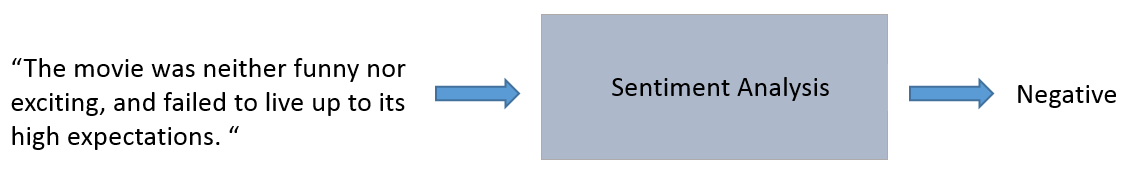
\includegraphics{Images/SentimentAnalysis.png}
\caption{caption}
\end{figure}

Ce genre de donnée peut être problèmatique. On ne peut jamais faire des
produit scalaire et des retropropagation sur des chaines de caractères .
Alors pour faciliter et rendre possible les différente opération sur ces
chaine de caractère on a pensé à convertir chaque mot dans les phrase
comme étant un vecteur.

\begin{figure}
\centering
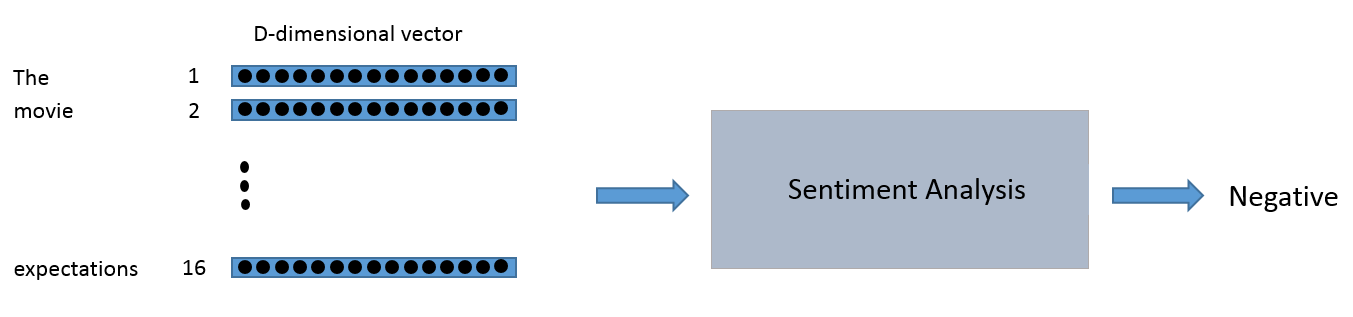
\includegraphics{Images/SentimentAnalysis2.png}
\caption{caption}
\end{figure}

On peux penser par exemple que l'input de notre text est une matrice de
16 dimensions.

    We want these vectors to be created in such a way that they somehow
represent the word and its context, meaning, and semantics. For example,
we'd like the vectors for the words ``love'' and ``adore'' to reside in
relatively the same area in the vector space since they both have
similar definitions and are both used in similar contexts. The vector
representation of a word is also known as a word embedding.

\begin{figure}
\centering
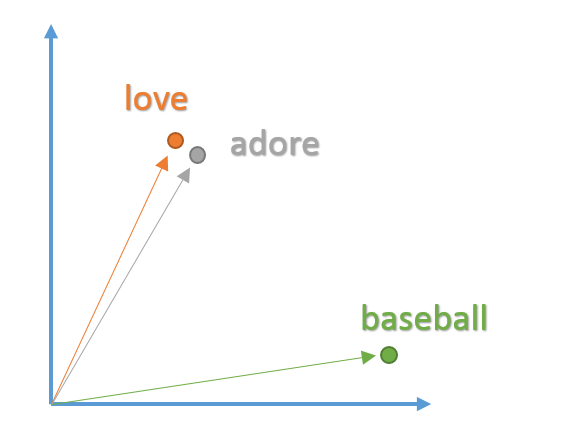
\includegraphics{Images/SentimentAnalysis8.png}
\caption{caption}
\end{figure}

    \section{Word2Vec}\label{word2vec}

    Nous voulons que ces vecteurs soient créés de telle manière qu'ils
représentent en quelque sorte le mot et son contexte, son sens et sa
sémantique. Par exemple, nous aimerions que les vecteurs pour les mots
«aimer» et «adorer» résident dans la même zone dans l'espace vectoriel,
car ils ont tous les deux des définitions similaires et sont tous deux
utilisés dans des contextes similaires. La représentation vectorielle
d'un mot est également connue sous le nom d'incorporation de mots.

\begin{figure}
\centering
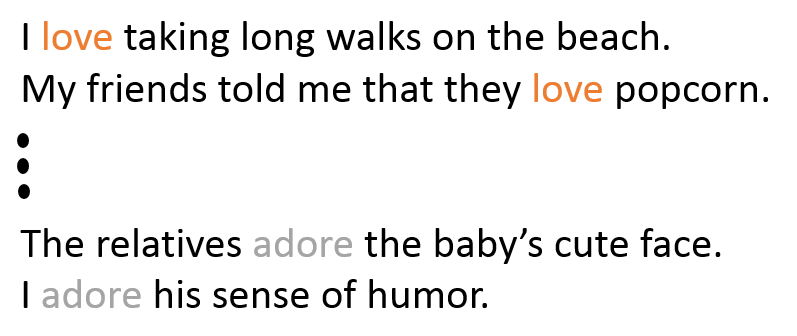
\includegraphics{Images/SentimentAnalysis9.png}
\caption{caption}
\end{figure}

Du contexte des phrases, nous pouvons voir que les deux mots sont
généralement utilisés dans des phrases avec des connotations positives
et précèdent généralement les noms ou les expressions nominales. C'est
une indication que les deux mots ont quelque chose en commun et peuvent
éventuellement être synonymes. Le contexte est également très important
lorsque l'on considère la structure grammaticale dans les phrases. La
plupart des phrases suivront les paradigmes traditionnels selon lesquels
les verbes suivent les noms, les adjectifs précèdent les noms, et ainsi
de suite. Pour cette raison, le modèle est plus susceptible de
positionner les noms dans la même zone générale que les autres noms. Le
modèle intègre un grand ensemble de phrases (Wikipédia en anglais par
exemple) et génère des vecteurs pour chaque mot unique du corpus. La
sortie d'un modèle Word2Vec s'appelle une matrice d'inclusion.

\begin{figure}
\centering
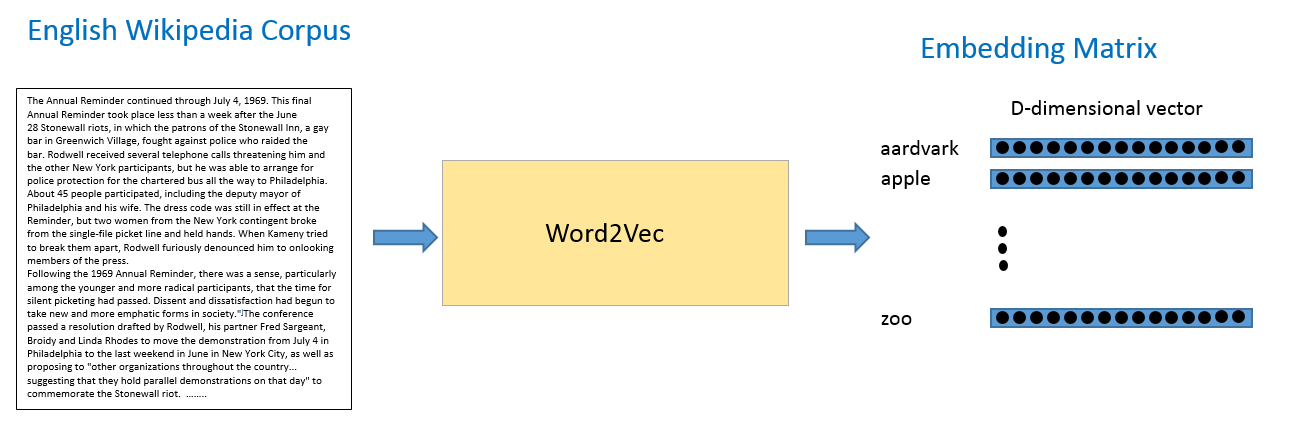
\includegraphics{Images/SentimentAnalysis3.png}
\caption{caption}
\end{figure}

Cette matrice d'inclusion contiendra des vecteurs pour chaque mot
distinct du corpus d'apprentissage. Traditionnellement, les matrices
d'inclusion peuvent contenir plus de 3 millions de vecteurs de mots.

Le modèle Word2Vec est entraîné en prenant chaque phrase dans l'ensemble
de données, en glissant une fenêtre de taille fixe dessus, et en
essayant de prédire le mot central de la fenêtre, étant donné les autres
mots. En utilisant une fonction de perte et une procédure
d'optimisation, le modèle génère des vecteurs pour chaque mot unique.
Les détails de cette procédure de formation peuvent être un peu
compliqués, donc nous allons passer à côté des détails pour l'instant,
mais la principale conclusion ici est que les entrées dans toute
approche Deep Learning d'une tâche NLP auront probablement des vecteurs
de mots en entrée.

    \section{Recurrent Neural Networks
(RNNs)}\label{recurrent-neural-networks-rnns}

    Maintenant que nous avons nos vecteurs de mot en entrée, regardons
l'architecture de réseau que nous allons construire. L'aspect unique des
données NLP est qu'il y a un aspect temporel. Chaque mot d'une phrase
dépend grandement de ce qui précède et vient après. Afin de rendre
compte de cette dépendance, nous utilisons un réseau de neurones
récurrent.

La structure du réseau neuronal récurrent est un peu différente de la NN
feedforward traditionnelle que vous pourriez être accosté à voir. Le
réseau feedforward se compose de noeuds d'entrée, d'unités cachées et de
noeuds de sortie.

\begin{figure}
\centering
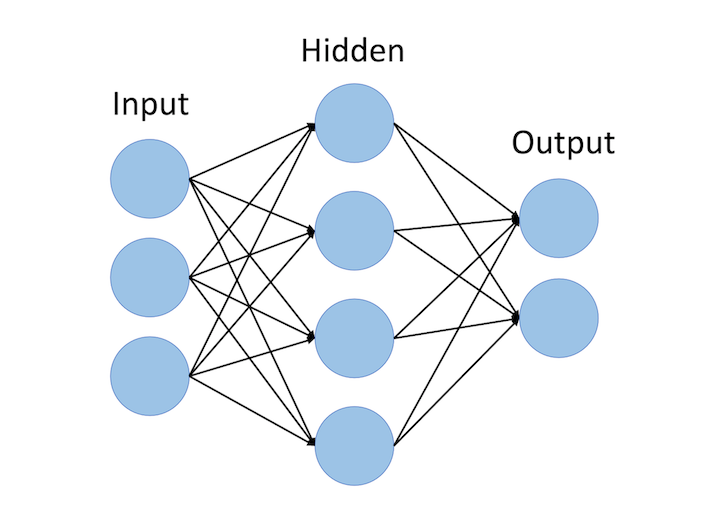
\includegraphics{Images/SentimentAnalysis17.png}
\caption{caption}
\end{figure}

La principale différence entre les réseaux de neurones feedforward et
récurrents est l'aspect temporel de ces derniers. Dans les RNN, chaque
mot d'une séquence d'entrée sera associé à un pas de temps spécifique.
En effet, le nombre de pas de temps sera égal à la longueur de séquence
maximale.

\begin{figure}
\centering

\includegraphics{Images/SentimentAnalysis18.png}
\caption{caption}
\end{figure}

Associé à chaque pas de temps est également un nouveau composant appelé
un vecteur hidden state h t . D'un niveau élevé, ce vecteur cherche à
encapsuler et résumer toutes les informations qui ont été vues dans les
étapes de temps précédentes. Tout comme x t est un vecteur qui encapsule
toutes les informations d'un mot spécifique, h t est un vecteur qui
résume les informations des étapes précédentes.

The hidden state est une fonction à la fois du vecteur de mot courant et
du vecteur d'état caché au pas de temps précédent. Le sigma indique que
la somme des deux termes passera par une fonction d'activation
(normalement un sigmoïde ou un tanh).

\begin{figure}
\centering
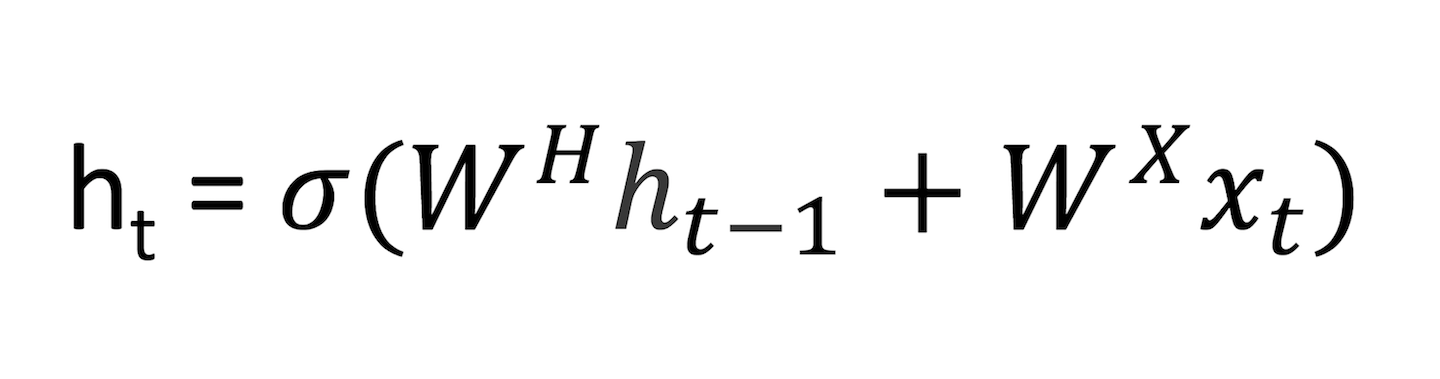
\includegraphics{Images/SentimentAnalysis15.png}
\caption{caption}
\end{figure}

Les 2 termes W dans la formulation ci-dessus représentent des matrices
de poids. Si vous regardez de près les superscripts, vous verrez qu'il y
a une matrice de poids W X que nous allons multiplier avec notre entrée,
et il y a une matrice de poids récurrente W H qui est multiplié avec le
vecteur d'hidden state de pas de temps précédent. W H est une matrice
qui reste la même pour tous les pas de temps, et la matrice de poids W X
est différente pour chaque entrée.

La magnitude de ces matrices de poids affecte la quantité que le vecteur
d'état caché est affecté par le vecteur courant ou l'état caché
précédent. Pour un exercice, jetez un oeil à la formule ci-dessus, et
considérez comment h t changerait si W X ou W H avaient de grandes ou
petites valeurs.

Regardons un exemple rapide. Lorsque la magnitude de W H est grande et
que la magnitude de W X est petite, on sait que h t est largement
affecté par h t-1 et non affecté par x t . En d'autres termes, le
vecteur d'état caché actuel voit que le mot courant est largement sans
conséquence sur le résumé global de la phrase, et il aura donc
essentiellement la même valeur que le vecteur au pas de temps précédent.

Les matrices de poids sont mises à jour grâce à un processus
d'optimisation appelé rétropropagation .

Le hidden state vector au dernier moment, le pas est introduit dans un
classificateur softmax binaire où il est multiplié par une autre matrice
de pondération et soumis à une fonction softmax qui produit des valeurs
entre 0 et 1, ce qui nous donne les probabilités de sentiment positif et
négatif.

\begin{figure}
\centering
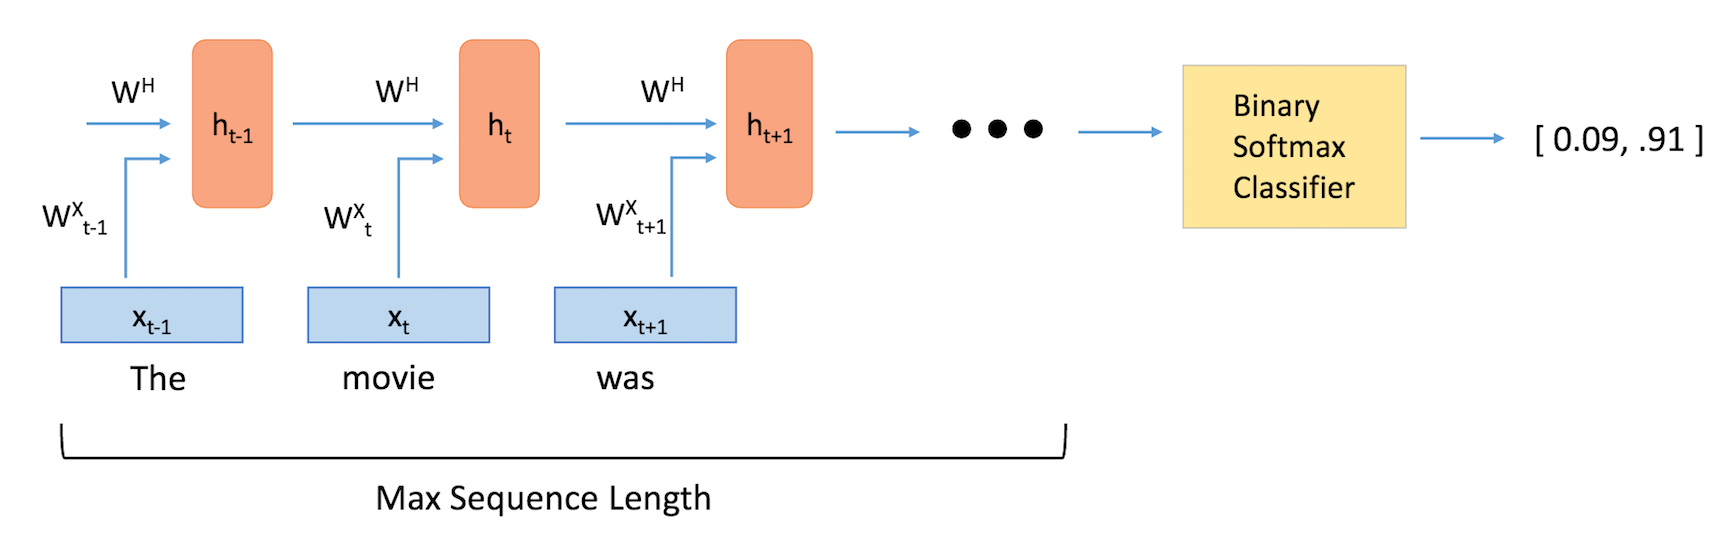
\includegraphics{Images/SentimentAnalysis16.png}
\caption{caption}
\end{figure}

    \section{Long Short Term Memory Units
(LSTMs)}\label{long-short-term-memory-units-lstms}

    Long Short Term Memory Units est un module que vous pouvez placer dans
des structures de réseaux de neurone reucrrent. À un niveau élevé, ils
s'assurent que le vecteur de hidden state h est capable d'encapsuler des
informations sur les dépendances à long terme dans le texte. Comme nous
l'avons vu dans la section précédente, la formulation pour h dans les
RNN traditionnels est relativement simple. Cette approche ne sera pas en
mesure de relier efficacement des informations séparées par plus de deux
pas de temps. Nous pouvons illustrer cette idée de gestion des
dépendances à long terme par un exemple dans le domaine de la réponse
aux questions. La fonction des modèles de réponse aux questions est de
prendre un passage de texte et de répondre à une question sur son
contenu. Regardons l'exemple suivant.

\begin{figure}
\centering
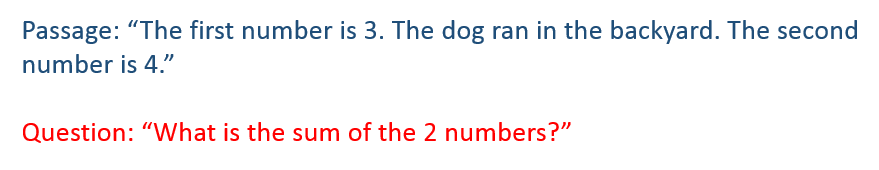
\includegraphics{Images/SentimentAnalysis4.png}
\caption{caption}
\end{figure}

Ici, nous voyons que la phrase du milieu n'a eu aucun impact sur la
question qui a été posée. Cependant, il existe un lien fort entre les
première et troisième phrases. Avec un RNN classique, le vecteur hidden
state à la fin du réseau pourrait avoir stocké plus d'informations sur
la phrase dog que sur la première phrase sur le nombre.
Fondamentalement, l'ajout d'unités LSTM permet de déterminer les
informations correctes et utiles qui doivent être stockées dans le
vecteur d'état caché.

En regardant les unités LSTM d'un point de vue plus technique, les
unités prennent le vecteur de mot courant x t et émettent le vecteur
d'état caché h t . Dans ces unités, la formulation de h t ser un peu
plus complexe que celle d'un RNN typique. Le calcul est décomposé en 4
composants, une porte d'entrée, une porte d'oubli (forget), une porte de
sortie et un nouveau conteneur de mémoire.

\begin{figure}
\centering
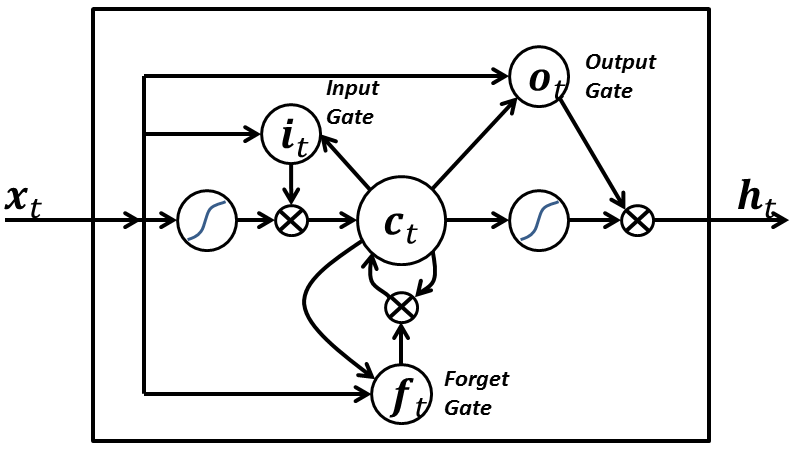
\includegraphics{Images/SentimentAnalysis10.png}
\caption{caption}
\end{figure}

Chaque porte prendra x t et h t-1 (non montré dans l'image) comme
entrées et effectuera un calcul sur celles-ci pour obtenir des états
intermédiaires. Chaque état intermédiaire est alimenté dans différents
pipelines et finalement l'information est agrégée pour former h t . Par
souci de simplicité, nous n'entrerons pas dans les formulations
spécifiques de chaque portail, mais il convient de noter que chacune de
ces portes peut être considérée comme différents modules au sein du LSTM
ayant chacun des fonctions différentes. La porte d'entrée détermine
combien d'accentuation mettre sur chacune des entrées, la porte d'oubli
détermine les informations que nous allons jeter, et la porte de sortie
détermine le h final t basé sur les états intermédiaires. Pour plus
d'informations sur la compréhension des fonctions des différentes portes
et les équations complètes, consultez Christopher Olah
\href{http://colah.github.io/posts/2015-08-Understanding-LSTMs/}{blog
post}.

En revenant sur le premier exemple avec la question "Quelle est la somme
des deux nombres?", Le modèle devrait être formé sur des types
similaires de questions et de réponses. Les unités LSTM seraient alors
capables de réaliser que toute phrase sans nombre n'aura probablement
pas d'impact sur la réponse à la question, et donc l'unité pourra
utiliser sa porte d'oubli pour jeter les informations inutiles sur le
chien, et plutôt Conservez les informations concernant les numéros.

    \section{Framing Sentiment Analysis as a Deep Learning
Problem}\label{framing-sentiment-analysis-as-a-deep-learning-problem}

    Comme mentionné précédemment, la tâche de l'analyse des sentiments
consiste à saisir une séquence d'entrée de mots et à déterminer si le
sentiment est positif, négatif ou neutre. Nous pouvons séparer cette
tâche spécifique (et la plupart des autres tâches PNL) en 5 composants
différents.

\begin{verbatim}
1) Formation d'un modèle de génération de vecteurs de mots (tel que Word2Vec) ou chargement de vecteurs de mots pré-assemblés
2) Création d'une matrice d'ID pour notre ensemble d'entraînement
3) Création de graphe RNN (avec unités LSTM)
4) Training
5) Test
\end{verbatim}

    \section{Loading Data}\label{loading-data}

    Premièrement, nous voulons créer nos vecteurs de mots. Pour simplifier,
nous allons utiliser un modèle pré-entraîné.

En tant que l'un des plus grandes entreprise de machine learning, Google
a pu former un modèle Word2Vec sur un ensemble de données Google News
qui contenait plus de 100 milliards de mots différents! De ce modèle,
Google
\href{https://code.google.com/archive/p/word2vec/\#Pre-trained_word_and_phrase_vectors}{a
pu entrain 3 million vecteur de mots}, chacun de dimentionnalité de 300.

Dans un scénario idéal, nous utiliserions ces vecteurs, mais comme la
matrice des vecteurs de mots est assez grande (3,6 Go!), Nous
utiliserons une matrice avec moin de taille qui est entraînée en
utilisant\href{http://nlp.stanford.edu/projects/glove/}{GloVe}, un
modèle de génération de vecteur de mot similaire. La matrice contiendra
400 000 vecteurs de mots, chacun ayant une dimension de 50.

Nous allons importer deux structures de données différentes, l'une sera
une liste Python avec les 400 000 mots, et l'autre sera une matrice
d'inclusion 400 000 x 50 qui contiendra toutes les valeurs de vecteur de
mots.

    \begin{Verbatim}[commandchars=\\\{\}]
{\color{incolor}In [{\color{incolor}1}]:} \PY{k+kn}{import} \PY{n+nn}{numpy} \PY{k}{as} \PY{n+nn}{np}
        \PY{n}{wordsList} \PY{o}{=} \PY{n}{np}\PY{o}{.}\PY{n}{load}\PY{p}{(}\PY{l+s+s1}{\PYZsq{}}\PY{l+s+s1}{wordsList.npy}\PY{l+s+s1}{\PYZsq{}}\PY{p}{)}
        \PY{n+nb}{print}\PY{p}{(}\PY{l+s+s1}{\PYZsq{}}\PY{l+s+s1}{Loaded the word list!}\PY{l+s+s1}{\PYZsq{}}\PY{p}{)}
        \PY{n}{wordsList} \PY{o}{=} \PY{n}{wordsList}\PY{o}{.}\PY{n}{tolist}\PY{p}{(}\PY{p}{)} \PY{c+c1}{\PYZsh{}Originally loaded as numpy array}
        \PY{n}{wordsList} \PY{o}{=} \PY{p}{[}\PY{n}{word}\PY{o}{.}\PY{n}{decode}\PY{p}{(}\PY{l+s+s1}{\PYZsq{}}\PY{l+s+s1}{UTF\PYZhy{}8}\PY{l+s+s1}{\PYZsq{}}\PY{p}{)} \PY{k}{for} \PY{n}{word} \PY{o+ow}{in} \PY{n}{wordsList}\PY{p}{]} \PY{c+c1}{\PYZsh{}Encode words as UTF\PYZhy{}8}
        \PY{n}{wordVectors} \PY{o}{=} \PY{n}{np}\PY{o}{.}\PY{n}{load}\PY{p}{(}\PY{l+s+s1}{\PYZsq{}}\PY{l+s+s1}{wordVectors.npy}\PY{l+s+s1}{\PYZsq{}}\PY{p}{)}
        \PY{n+nb}{print} \PY{p}{(}\PY{l+s+s1}{\PYZsq{}}\PY{l+s+s1}{Loaded the word vectors!}\PY{l+s+s1}{\PYZsq{}}\PY{p}{)}
\end{Verbatim}


    \begin{Verbatim}[commandchars=\\\{\}]
Loaded the word list!
Loaded the word vectors!

    \end{Verbatim}

    Juste pour s'assurer que tout a été correctement chargé, nous pouvons
regarder les dimensions de la liste de vocabulaire et de la matrice
d'intégration.

    \begin{Verbatim}[commandchars=\\\{\}]
{\color{incolor}In [{\color{incolor}2}]:} \PY{n+nb}{print}\PY{p}{(}\PY{n+nb}{len}\PY{p}{(}\PY{n}{wordsList}\PY{p}{)}\PY{p}{)}
        \PY{n+nb}{print}\PY{p}{(}\PY{n}{wordVectors}\PY{o}{.}\PY{n}{shape}\PY{p}{)}
\end{Verbatim}


    \begin{Verbatim}[commandchars=\\\{\}]
400000
(400000, 50)

    \end{Verbatim}

    Nous pouvons également chercher dans notre liste de mots un mot comme
"baseball", puis accéder à son vecteur correspondant à travers la
matrice d'intégration.

    \begin{Verbatim}[commandchars=\\\{\}]
{\color{incolor}In [{\color{incolor}3}]:} \PY{n}{baseballIndex} \PY{o}{=} \PY{n}{wordsList}\PY{o}{.}\PY{n}{index}\PY{p}{(}\PY{l+s+s1}{\PYZsq{}}\PY{l+s+s1}{baseball}\PY{l+s+s1}{\PYZsq{}}\PY{p}{)}
        \PY{n}{wordVectors}\PY{p}{[}\PY{n}{baseballIndex}\PY{p}{]}
\end{Verbatim}


\begin{Verbatim}[commandchars=\\\{\}]
{\color{outcolor}Out[{\color{outcolor}3}]:} array([-1.93270004,  1.04209995, -0.78514999,  0.91033   ,  0.22711   ,
               -0.62158   , -1.64929998,  0.07686   , -0.58679998,  0.058831  ,
                0.35628   ,  0.68915999, -0.50598001,  0.70472997,  1.26639998,
               -0.40031001, -0.020687  ,  0.80862999, -0.90565997, -0.074054  ,
               -0.87674999, -0.62910002, -0.12684999,  0.11524   , -0.55685002,
               -1.68260002, -0.26291001,  0.22632   ,  0.713     , -1.08280003,
                2.12310004,  0.49869001,  0.066711  , -0.48225999, -0.17896999,
                0.47699001,  0.16384   ,  0.16537   , -0.11506   , -0.15962   ,
               -0.94926   , -0.42833   , -0.59456998,  1.35660005, -0.27506   ,
                0.19918001, -0.36008   ,  0.55667001, -0.70314997,  0.17157   ], dtype=float32)
\end{Verbatim}
            
    Maintenant que nous avons nos vecteurs, notre première étape consiste à
prendre une phrase d'entrée puis à construire la représentation de son
vecteur. Disons que nous avons la phrase d'entrée "Je pensais que le
film était incroyable et inspirant". Pour obtenir les vecteurs de mots,
nous pouvons utiliser la fonction de recherche d'intégration de
Tensorflow. Cette fonction prend deux arguments, un pour la matrice
d'intégration (la matrice wordVectors dans notre cas) et un pour les
identifiants de chacun des mots. Le vecteur ids peut être considéré
comme la représentation entière de l'ensemble d'apprentissage. C'est
fondamentalement juste l'index de ligne de chacun des mots. Regardons un
exemple rapide pour rendre cela concret.

    \begin{Verbatim}[commandchars=\\\{\}]
{\color{incolor}In [{\color{incolor}4}]:} \PY{k+kn}{import} \PY{n+nn}{tensorflow} \PY{k}{as} \PY{n+nn}{tf}
        \PY{n}{maxSeqLength} \PY{o}{=} \PY{l+m+mi}{10} \PY{c+c1}{\PYZsh{}Maximum length of sentence}
        \PY{n}{numDimensions} \PY{o}{=} \PY{l+m+mi}{300} \PY{c+c1}{\PYZsh{}Dimensions for each word vector}
        \PY{n}{firstSentence} \PY{o}{=} \PY{n}{np}\PY{o}{.}\PY{n}{zeros}\PY{p}{(}\PY{p}{(}\PY{n}{maxSeqLength}\PY{p}{)}\PY{p}{,} \PY{n}{dtype}\PY{o}{=}\PY{l+s+s1}{\PYZsq{}}\PY{l+s+s1}{int32}\PY{l+s+s1}{\PYZsq{}}\PY{p}{)}
        \PY{n}{firstSentence}\PY{p}{[}\PY{l+m+mi}{0}\PY{p}{]} \PY{o}{=} \PY{n}{wordsList}\PY{o}{.}\PY{n}{index}\PY{p}{(}\PY{l+s+s2}{\PYZdq{}}\PY{l+s+s2}{i}\PY{l+s+s2}{\PYZdq{}}\PY{p}{)}
        \PY{n}{firstSentence}\PY{p}{[}\PY{l+m+mi}{1}\PY{p}{]} \PY{o}{=} \PY{n}{wordsList}\PY{o}{.}\PY{n}{index}\PY{p}{(}\PY{l+s+s2}{\PYZdq{}}\PY{l+s+s2}{thought}\PY{l+s+s2}{\PYZdq{}}\PY{p}{)}
        \PY{n}{firstSentence}\PY{p}{[}\PY{l+m+mi}{2}\PY{p}{]} \PY{o}{=} \PY{n}{wordsList}\PY{o}{.}\PY{n}{index}\PY{p}{(}\PY{l+s+s2}{\PYZdq{}}\PY{l+s+s2}{the}\PY{l+s+s2}{\PYZdq{}}\PY{p}{)}
        \PY{n}{firstSentence}\PY{p}{[}\PY{l+m+mi}{3}\PY{p}{]} \PY{o}{=} \PY{n}{wordsList}\PY{o}{.}\PY{n}{index}\PY{p}{(}\PY{l+s+s2}{\PYZdq{}}\PY{l+s+s2}{movie}\PY{l+s+s2}{\PYZdq{}}\PY{p}{)}
        \PY{n}{firstSentence}\PY{p}{[}\PY{l+m+mi}{4}\PY{p}{]} \PY{o}{=} \PY{n}{wordsList}\PY{o}{.}\PY{n}{index}\PY{p}{(}\PY{l+s+s2}{\PYZdq{}}\PY{l+s+s2}{was}\PY{l+s+s2}{\PYZdq{}}\PY{p}{)}
        \PY{n}{firstSentence}\PY{p}{[}\PY{l+m+mi}{5}\PY{p}{]} \PY{o}{=} \PY{n}{wordsList}\PY{o}{.}\PY{n}{index}\PY{p}{(}\PY{l+s+s2}{\PYZdq{}}\PY{l+s+s2}{incredible}\PY{l+s+s2}{\PYZdq{}}\PY{p}{)}
        \PY{n}{firstSentence}\PY{p}{[}\PY{l+m+mi}{6}\PY{p}{]} \PY{o}{=} \PY{n}{wordsList}\PY{o}{.}\PY{n}{index}\PY{p}{(}\PY{l+s+s2}{\PYZdq{}}\PY{l+s+s2}{and}\PY{l+s+s2}{\PYZdq{}}\PY{p}{)}
        \PY{n}{firstSentence}\PY{p}{[}\PY{l+m+mi}{7}\PY{p}{]} \PY{o}{=} \PY{n}{wordsList}\PY{o}{.}\PY{n}{index}\PY{p}{(}\PY{l+s+s2}{\PYZdq{}}\PY{l+s+s2}{inspiring}\PY{l+s+s2}{\PYZdq{}}\PY{p}{)}
        \PY{c+c1}{\PYZsh{}firstSentence[8] and firstSentence[9] are going to be 0}
        \PY{n+nb}{print}\PY{p}{(}\PY{n}{firstSentence}\PY{o}{.}\PY{n}{shape}\PY{p}{)}
        \PY{n+nb}{print}\PY{p}{(}\PY{n}{firstSentence}\PY{p}{)} \PY{c+c1}{\PYZsh{}Shows the row index for each word}
\end{Verbatim}


    \begin{Verbatim}[commandchars=\\\{\}]
(10,)
[    41    804 201534   1005     15   7446      5  13767      0      0]

    \end{Verbatim}

    le pipeline de données peut être représenté ainsi.

    \begin{figure}
\centering
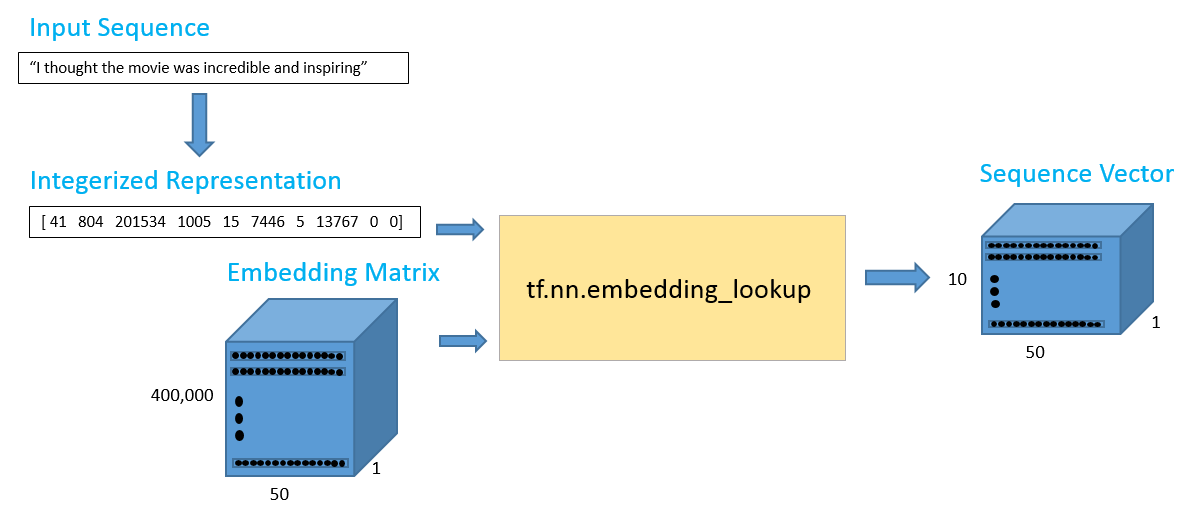
\includegraphics{Images/SentimentAnalysis5.png}
\caption{caption}
\end{figure}

    La sortie 10 x 50 doit contenir les vecteurs de mot 50 dimensions pour
chacun des 10 mots de la séquence.

    \begin{Verbatim}[commandchars=\\\{\}]
{\color{incolor}In [{\color{incolor}14}]:} \PY{k}{with} \PY{n}{tf}\PY{o}{.}\PY{n}{Session}\PY{p}{(}\PY{p}{)} \PY{k}{as} \PY{n}{sess}\PY{p}{:}
             \PY{n+nb}{print}\PY{p}{(}\PY{n}{tf}\PY{o}{.}\PY{n}{nn}\PY{o}{.}\PY{n}{embedding\PYZus{}lookup}\PY{p}{(}\PY{n}{wordVectors}\PY{p}{,}\PY{n}{firstSentence}\PY{p}{)}\PY{o}{.}\PY{n}{eval}\PY{p}{(}\PY{p}{)}\PY{o}{.}\PY{n}{shape}\PY{p}{)}
\end{Verbatim}


    \begin{Verbatim}[commandchars=\\\{\}]
(10, 50)

    \end{Verbatim}

    Avant de créer la matrice d'identifiants pour l'ensemble de l'ensemble
de formation, prenons d'abord un certain temps pour visualiser le type
de données que nous avons. Cela nous aidera à déterminer la meilleure
valeur pour définir notre longueur de séquence maximale. Dans l'exemple
précédent, nous avons utilisé une longueur maximale de 10, mais cette
valeur dépend largement des entrées que vous avez.

    Le dataset que nous allons utiliser est le jeu de données de review de
Amazon food. Cet ensemble compte 35173 critiques de films, avec
critiques positives et 25 087 critiques positives. Chacune des critiques
est stockée dans un fichier txt que nous devons analyser. Les
commentaires négatives sont stockés dans un répertoire et les avis
négatifs sont stockés dans un autre. Le morceau de code suivant
déterminera le nombre total et moyen de mots dans chaque révision.

    \begin{Verbatim}[commandchars=\\\{\}]
{\color{incolor}In [{\color{incolor}6}]:} \PY{k+kn}{from} \PY{n+nn}{os} \PY{k}{import} \PY{n}{listdir}
        \PY{k+kn}{from} \PY{n+nn}{os}\PY{n+nn}{.}\PY{n+nn}{path} \PY{k}{import} \PY{n}{isfile}\PY{p}{,} \PY{n}{join}
        \PY{n}{positiveFiles} \PY{o}{=} \PY{p}{[}\PY{l+s+s1}{\PYZsq{}}\PY{l+s+s1}{positiveReviews/}\PY{l+s+s1}{\PYZsq{}} \PY{o}{+} \PY{n}{f} \PY{k}{for} \PY{n}{f} \PY{o+ow}{in} \PY{n}{listdir}\PY{p}{(}\PY{l+s+s1}{\PYZsq{}}\PY{l+s+s1}{positiveReviews/}\PY{l+s+s1}{\PYZsq{}}\PY{p}{)} \PY{k}{if} \PY{n}{isfile}\PY{p}{(}\PY{n}{join}\PY{p}{(}\PY{l+s+s1}{\PYZsq{}}\PY{l+s+s1}{positiveReviews/}\PY{l+s+s1}{\PYZsq{}}\PY{p}{,} \PY{n}{f}\PY{p}{)}\PY{p}{)}\PY{p}{]}
        \PY{n}{negativeFiles} \PY{o}{=} \PY{p}{[}\PY{l+s+s1}{\PYZsq{}}\PY{l+s+s1}{negativeReviews/}\PY{l+s+s1}{\PYZsq{}} \PY{o}{+} \PY{n}{f} \PY{k}{for} \PY{n}{f} \PY{o+ow}{in} \PY{n}{listdir}\PY{p}{(}\PY{l+s+s1}{\PYZsq{}}\PY{l+s+s1}{negativeReviews/}\PY{l+s+s1}{\PYZsq{}}\PY{p}{)} \PY{k}{if} \PY{n}{isfile}\PY{p}{(}\PY{n}{join}\PY{p}{(}\PY{l+s+s1}{\PYZsq{}}\PY{l+s+s1}{negativeReviews/}\PY{l+s+s1}{\PYZsq{}}\PY{p}{,} \PY{n}{f}\PY{p}{)}\PY{p}{)}\PY{p}{]}
        \PY{n}{numWords} \PY{o}{=} \PY{p}{[}\PY{p}{]}
        \PY{k}{for} \PY{n}{pf} \PY{o+ow}{in} \PY{n}{positiveFiles}\PY{p}{:}
            \PY{k}{with} \PY{n+nb}{open}\PY{p}{(}\PY{n}{pf}\PY{p}{,} \PY{l+s+s2}{\PYZdq{}}\PY{l+s+s2}{r}\PY{l+s+s2}{\PYZdq{}}\PY{p}{,} \PY{n}{encoding}\PY{o}{=}\PY{l+s+s1}{\PYZsq{}}\PY{l+s+s1}{utf\PYZhy{}8}\PY{l+s+s1}{\PYZsq{}}\PY{p}{)} \PY{k}{as} \PY{n}{f}\PY{p}{:}
                \PY{n}{line}\PY{o}{=}\PY{n}{f}\PY{o}{.}\PY{n}{readline}\PY{p}{(}\PY{p}{)}
                \PY{n}{counter} \PY{o}{=} \PY{n+nb}{len}\PY{p}{(}\PY{n}{line}\PY{o}{.}\PY{n}{split}\PY{p}{(}\PY{p}{)}\PY{p}{)}
                \PY{n}{numWords}\PY{o}{.}\PY{n}{append}\PY{p}{(}\PY{n}{counter}\PY{p}{)}       
        \PY{n+nb}{print}\PY{p}{(}\PY{l+s+s1}{\PYZsq{}}\PY{l+s+s1}{Positive files finished}\PY{l+s+s1}{\PYZsq{}}\PY{p}{)}
        
        \PY{k}{for} \PY{n}{nf} \PY{o+ow}{in} \PY{n}{negativeFiles}\PY{p}{:}
            \PY{k}{with} \PY{n+nb}{open}\PY{p}{(}\PY{n}{nf}\PY{p}{,} \PY{l+s+s2}{\PYZdq{}}\PY{l+s+s2}{r}\PY{l+s+s2}{\PYZdq{}}\PY{p}{,} \PY{n}{encoding}\PY{o}{=}\PY{l+s+s1}{\PYZsq{}}\PY{l+s+s1}{utf\PYZhy{}8}\PY{l+s+s1}{\PYZsq{}}\PY{p}{)} \PY{k}{as} \PY{n}{f}\PY{p}{:}
                \PY{n}{line}\PY{o}{=}\PY{n}{f}\PY{o}{.}\PY{n}{readline}\PY{p}{(}\PY{p}{)}
                \PY{n}{counter} \PY{o}{=} \PY{n+nb}{len}\PY{p}{(}\PY{n}{line}\PY{o}{.}\PY{n}{split}\PY{p}{(}\PY{p}{)}\PY{p}{)}
                \PY{n}{numWords}\PY{o}{.}\PY{n}{append}\PY{p}{(}\PY{n}{counter}\PY{p}{)}  
        \PY{n+nb}{print}\PY{p}{(}\PY{l+s+s1}{\PYZsq{}}\PY{l+s+s1}{Negative files finished}\PY{l+s+s1}{\PYZsq{}}\PY{p}{)}
        
        \PY{n}{numFiles} \PY{o}{=} \PY{n+nb}{len}\PY{p}{(}\PY{n}{numWords}\PY{p}{)}
        \PY{n+nb}{print}\PY{p}{(}\PY{l+s+s1}{\PYZsq{}}\PY{l+s+s1}{The total number of files is}\PY{l+s+s1}{\PYZsq{}}\PY{p}{,} \PY{n}{numFiles}\PY{p}{)}
        \PY{n+nb}{print}\PY{p}{(}\PY{l+s+s1}{\PYZsq{}}\PY{l+s+s1}{The total number of words in the files is}\PY{l+s+s1}{\PYZsq{}}\PY{p}{,} \PY{n+nb}{sum}\PY{p}{(}\PY{n}{numWords}\PY{p}{)}\PY{p}{)}
        \PY{n+nb}{print}\PY{p}{(}\PY{l+s+s1}{\PYZsq{}}\PY{l+s+s1}{The average number of words in the files is}\PY{l+s+s1}{\PYZsq{}}\PY{p}{,} \PY{n+nb}{sum}\PY{p}{(}\PY{n}{numWords}\PY{p}{)}\PY{o}{/}\PY{n+nb}{len}\PY{p}{(}\PY{n}{numWords}\PY{p}{)}\PY{p}{)}
\end{Verbatim}


    \begin{Verbatim}[commandchars=\\\{\}]
Positive files finished
Negative files finished
The total number of files is 35173
The total number of words in the files is 2713530
The average number of words in the files is 77.14809655133199

    \end{Verbatim}

    Nous pouvons également utiliser la bibliothèque Matplot pour visualiser
ces données dans un format d'histogramme.

    \begin{Verbatim}[commandchars=\\\{\}]
{\color{incolor}In [{\color{incolor}7}]:} \PY{k+kn}{import} \PY{n+nn}{matplotlib}\PY{n+nn}{.}\PY{n+nn}{pyplot} \PY{k}{as} \PY{n+nn}{plt}
        \PY{o}{\PYZpc{}}\PY{k}{matplotlib} inline
        \PY{n}{plt}\PY{o}{.}\PY{n}{hist}\PY{p}{(}\PY{n}{numWords}\PY{p}{,} \PY{l+m+mi}{50}\PY{p}{)}
        \PY{n}{plt}\PY{o}{.}\PY{n}{xlabel}\PY{p}{(}\PY{l+s+s1}{\PYZsq{}}\PY{l+s+s1}{Sequence Length}\PY{l+s+s1}{\PYZsq{}}\PY{p}{)}
        \PY{n}{plt}\PY{o}{.}\PY{n}{ylabel}\PY{p}{(}\PY{l+s+s1}{\PYZsq{}}\PY{l+s+s1}{Frequency}\PY{l+s+s1}{\PYZsq{}}\PY{p}{)}
        \PY{n}{plt}\PY{o}{.}\PY{n}{axis}\PY{p}{(}\PY{p}{[}\PY{l+m+mi}{0}\PY{p}{,} \PY{l+m+mi}{1200}\PY{p}{,} \PY{l+m+mi}{0}\PY{p}{,} \PY{l+m+mi}{8000}\PY{p}{]}\PY{p}{)}
        \PY{n}{plt}\PY{o}{.}\PY{n}{show}\PY{p}{(}\PY{p}{)}
\end{Verbatim}


    \begin{center}
    \adjustimage{max size={0.9\linewidth}{0.9\paperheight}}{output_30_0.png}
    \end{center}
    { \hspace*{\fill} \\}
    
    A partir de l'histogramme ainsi que du nombre moyen de mots par fichier,
nous pouvons affirmer que la plupart des révisions tomberont sous 80
mots, on choisit alors la longueur de message de 150.

    \begin{Verbatim}[commandchars=\\\{\}]
{\color{incolor}In [{\color{incolor}8}]:} \PY{n}{maxSeqLength} \PY{o}{=} \PY{l+m+mi}{150}
\end{Verbatim}


    Voyons comment nous pouvons prendre un seul fichier et le transformer en
notre matrice d'identifiants. C'est ce que l'un des commentaires
ressemble au format de fichier texte.

    \begin{Verbatim}[commandchars=\\\{\}]
{\color{incolor}In [{\color{incolor}9}]:} \PY{n}{fname} \PY{o}{=} \PY{n}{positiveFiles}\PY{p}{[}\PY{l+m+mi}{3}\PY{p}{]} \PY{c+c1}{\PYZsh{}Can use any valid index (not just 3)}
        \PY{k}{with} \PY{n+nb}{open}\PY{p}{(}\PY{n}{fname}\PY{p}{)} \PY{k}{as} \PY{n}{f}\PY{p}{:}
            \PY{k}{for} \PY{n}{lines} \PY{o+ow}{in} \PY{n}{f}\PY{p}{:}
                \PY{n+nb}{print}\PY{p}{(}\PY{n}{lines}\PY{p}{)}
                \PY{n}{exit}
\end{Verbatim}


    \begin{Verbatim}[commandchars=\\\{\}]
We started using ghee in place of oils to help our daughter with severe autism.  She appears to be in better health and mood since this change.  We have tried four different varieties of ghee, but this is the best tasting and fits into more recipes because of the mild taste. There is a big price difference, but this  and is worth the extra money.

    \end{Verbatim}

    Maintenant, convertissons en une matrice d'identifiants

    \begin{Verbatim}[commandchars=\\\{\}]
{\color{incolor}In [{\color{incolor}10}]:} \PY{c+c1}{\PYZsh{} Removes punctuation, parentheses, question marks, etc., and leaves only alphanumeric characters}
         \PY{k+kn}{import} \PY{n+nn}{re}
         \PY{n}{strip\PYZus{}special\PYZus{}chars} \PY{o}{=} \PY{n}{re}\PY{o}{.}\PY{n}{compile}\PY{p}{(}\PY{l+s+s2}{\PYZdq{}}\PY{l+s+s2}{[\PYZca{}A\PYZhy{}Za\PYZhy{}z0\PYZhy{}9 ]+}\PY{l+s+s2}{\PYZdq{}}\PY{p}{)}
         
         \PY{k}{def} \PY{n+nf}{cleanSentences}\PY{p}{(}\PY{n}{string}\PY{p}{)}\PY{p}{:}
             \PY{n}{string} \PY{o}{=} \PY{n}{string}\PY{o}{.}\PY{n}{lower}\PY{p}{(}\PY{p}{)}\PY{o}{.}\PY{n}{replace}\PY{p}{(}\PY{l+s+s2}{\PYZdq{}}\PY{l+s+s2}{\PYZlt{}br /\PYZgt{}}\PY{l+s+s2}{\PYZdq{}}\PY{p}{,} \PY{l+s+s2}{\PYZdq{}}\PY{l+s+s2}{ }\PY{l+s+s2}{\PYZdq{}}\PY{p}{)}
             \PY{k}{return} \PY{n}{re}\PY{o}{.}\PY{n}{sub}\PY{p}{(}\PY{n}{strip\PYZus{}special\PYZus{}chars}\PY{p}{,} \PY{l+s+s2}{\PYZdq{}}\PY{l+s+s2}{\PYZdq{}}\PY{p}{,} \PY{n}{string}\PY{o}{.}\PY{n}{lower}\PY{p}{(}\PY{p}{)}\PY{p}{)}
\end{Verbatim}


    \begin{Verbatim}[commandchars=\\\{\}]
{\color{incolor}In [{\color{incolor}11}]:} \PY{n}{firstFile} \PY{o}{=} \PY{n}{np}\PY{o}{.}\PY{n}{zeros}\PY{p}{(}\PY{p}{(}\PY{n}{maxSeqLength}\PY{p}{)}\PY{p}{,} \PY{n}{dtype}\PY{o}{=}\PY{l+s+s1}{\PYZsq{}}\PY{l+s+s1}{int32}\PY{l+s+s1}{\PYZsq{}}\PY{p}{)}
         \PY{k}{with} \PY{n+nb}{open}\PY{p}{(}\PY{n}{fname}\PY{p}{)} \PY{k}{as} \PY{n}{f}\PY{p}{:}
             \PY{n}{indexCounter} \PY{o}{=} \PY{l+m+mi}{0}
             \PY{n}{line}\PY{o}{=}\PY{n}{f}\PY{o}{.}\PY{n}{readline}\PY{p}{(}\PY{p}{)}
             \PY{n}{cleanedLine} \PY{o}{=} \PY{n}{cleanSentences}\PY{p}{(}\PY{n}{line}\PY{p}{)}
             \PY{n}{split} \PY{o}{=} \PY{n}{cleanedLine}\PY{o}{.}\PY{n}{split}\PY{p}{(}\PY{p}{)}
             \PY{k}{for} \PY{n}{word} \PY{o+ow}{in} \PY{n}{split}\PY{p}{:}
                 \PY{k}{try}\PY{p}{:}
                     \PY{n}{firstFile}\PY{p}{[}\PY{n}{indexCounter}\PY{p}{]} \PY{o}{=} \PY{n}{wordsList}\PY{o}{.}\PY{n}{index}\PY{p}{(}\PY{n}{word}\PY{p}{)}
                 \PY{k}{except} \PY{n+ne}{ValueError}\PY{p}{:}
                     \PY{n}{firstFile}\PY{p}{[}\PY{n}{indexCounter}\PY{p}{]} \PY{o}{=} \PY{l+m+mi}{399999} \PY{c+c1}{\PYZsh{}Vector for unknown words}
                 \PY{n}{indexCounter} \PY{o}{=} \PY{n}{indexCounter} \PY{o}{+} \PY{l+m+mi}{1}
         \PY{n}{firstFile}
\end{Verbatim}


\begin{Verbatim}[commandchars=\\\{\}]
{\color{outcolor}Out[{\color{outcolor}11}]:} array([    53,    551,    622,  68774,      6,    241,      3,  16237,
                     4,    275,    162,   1131,     17,   2546,  17179,     67,
                  1658,      4,     30,      6,    439,    360,      5,   5030,
                   108,     37,    511,     53,     33,    977,    133,    494,
                  8576,      3,  68774,     34,     37,     14, 201534,    254,
                 16701,      5,  10094,     75,     56,   8628,    113,      3,
                201534,   6715,   4374,     63,     14,      7,    365,    626,
                  2333,     34,     37,      5,     14,   1089, 201534,   2004,
                   308,      0,      0,      0,      0,      0,      0,      0,
                     0,      0,      0,      0,      0,      0,      0,      0,
                     0,      0,      0,      0,      0,      0,      0,      0,
                     0,      0,      0,      0,      0,      0,      0,      0,
                     0,      0,      0,      0,      0,      0,      0,      0,
                     0,      0,      0,      0,      0,      0,      0,      0,
                     0,      0,      0,      0,      0,      0,      0,      0,
                     0,      0,      0,      0,      0,      0,      0,      0,
                     0,      0,      0,      0,      0,      0,      0,      0,
                     0,      0,      0,      0,      0,      0,      0,      0,
                     0,      0,      0,      0,      0,      0], dtype=int32)
\end{Verbatim}
            
    Maintenant, faisons la même chose pour chacun de nos 35173 avis. Nous
chargerons dans l'ensemble de formation de film et l'integerize pour
obtenir une matrice 35173 x 150. C'était un processus coûteux en calcul,
donc au lieu de vous faire exécuter toute la pièce, nous allons charger
dans une matrice d'ID pré-calculée.

    \begin{Verbatim}[commandchars=\\\{\}]
{\color{incolor}In [{\color{incolor} }]:} \PY{c+c1}{\PYZsh{} ids = np.zeros((numFiles, maxSeqLength), dtype=\PYZsq{}int32\PYZsq{})}
        \PY{c+c1}{\PYZsh{} fileCounter = 0}
        \PY{c+c1}{\PYZsh{} for pf in positiveFiles:}
        \PY{c+c1}{\PYZsh{}    with open(pf, \PYZdq{}r\PYZdq{}) as f:}
        \PY{c+c1}{\PYZsh{}        indexCounter = 0}
        \PY{c+c1}{\PYZsh{}        line=f.readline()}
        \PY{c+c1}{\PYZsh{}        cleanedLine = cleanSentences(line)}
        \PY{c+c1}{\PYZsh{}        split = cleanedLine.split()}
        \PY{c+c1}{\PYZsh{}        for word in split:}
        \PY{c+c1}{\PYZsh{}            try:}
        \PY{c+c1}{\PYZsh{}                ids[fileCounter][indexCounter] = wordsList.index(word)}
        \PY{c+c1}{\PYZsh{}            except ValueError:}
        \PY{c+c1}{\PYZsh{}                ids[fileCounter][indexCounter] = 399999 \PYZsh{}Vector for unkown words}
        \PY{c+c1}{\PYZsh{}            indexCounter = indexCounter + 1}
        \PY{c+c1}{\PYZsh{}            if indexCounter \PYZgt{}= maxSeqLength:}
        \PY{c+c1}{\PYZsh{}                break}
        \PY{c+c1}{\PYZsh{}        fileCounter = fileCounter + 1 }
        \PY{c+c1}{\PYZsh{}}
        \PY{c+c1}{\PYZsh{} for nf in negativeFiles:}
        \PY{c+c1}{\PYZsh{}    with open(nf, \PYZdq{}r\PYZdq{}) as f:}
        \PY{c+c1}{\PYZsh{}        indexCounter = 0}
        \PY{c+c1}{\PYZsh{}        line=f.readline()}
        \PY{c+c1}{\PYZsh{}        cleanedLine = cleanSentences(line)}
        \PY{c+c1}{\PYZsh{}        split = cleanedLine.split()}
        \PY{c+c1}{\PYZsh{}        for word in split:}
        \PY{c+c1}{\PYZsh{}            try:}
        \PY{c+c1}{\PYZsh{}                ids[fileCounter][indexCounter] = wordsList.index(word)}
        \PY{c+c1}{\PYZsh{}            except ValueError:}
        \PY{c+c1}{\PYZsh{}                ids[fileCounter][indexCounter] = 399999 \PYZsh{}Vector for unkown words}
        \PY{c+c1}{\PYZsh{}            indexCounter = indexCounter + 1}
        \PY{c+c1}{\PYZsh{}            if indexCounter \PYZgt{}= maxSeqLength:}
        \PY{c+c1}{\PYZsh{}                break}
        \PY{c+c1}{\PYZsh{}        fileCounter = fileCounter + 1 }
         \PY{c+c1}{\PYZsh{}Pass into embedding function and see if it evaluates. }
        
        \PY{c+c1}{\PYZsh{} np.save(\PYZsq{}idsMatrix\PYZsq{}, ids)}
\end{Verbatim}


    \begin{Verbatim}[commandchars=\\\{\}]
{\color{incolor}In [{\color{incolor}12}]:} \PY{n}{ids} \PY{o}{=} \PY{n}{np}\PY{o}{.}\PY{n}{load}\PY{p}{(}\PY{l+s+s1}{\PYZsq{}}\PY{l+s+s1}{idsMatrix.npy}\PY{l+s+s1}{\PYZsq{}}\PY{p}{)}
\end{Verbatim}


    \section{Helper Functions}\label{helper-functions}

    Vous trouverez ci-dessous quelques fonctions auxiliaires utiles lors de
la formation ultérieure du réseau.

    \begin{Verbatim}[commandchars=\\\{\}]
{\color{incolor}In [{\color{incolor}13}]:} \PY{k+kn}{from} \PY{n+nn}{random} \PY{k}{import} \PY{n}{randint}
         
         \PY{k}{def} \PY{n+nf}{getTrainBatch}\PY{p}{(}\PY{p}{)}\PY{p}{:}
             \PY{n}{labels} \PY{o}{=} \PY{p}{[}\PY{p}{]}
             \PY{n}{arr} \PY{o}{=} \PY{n}{np}\PY{o}{.}\PY{n}{zeros}\PY{p}{(}\PY{p}{[}\PY{n}{batchSize}\PY{p}{,} \PY{n}{maxSeqLength}\PY{p}{]}\PY{p}{)}
             \PY{k}{for} \PY{n}{i} \PY{o+ow}{in} \PY{n+nb}{range}\PY{p}{(}\PY{n}{batchSize}\PY{p}{)}\PY{p}{:}
                 \PY{k}{if} \PY{p}{(}\PY{n}{i} \PY{o}{\PYZpc{}} \PY{l+m+mi}{2} \PY{o}{==} \PY{l+m+mi}{0}\PY{p}{)}\PY{p}{:} 
                     \PY{n}{num} \PY{o}{=} \PY{n}{randint}\PY{p}{(}\PY{l+m+mi}{1}\PY{p}{,}\PY{l+m+mi}{25087}\PY{p}{)}
                     \PY{n}{labels}\PY{o}{.}\PY{n}{append}\PY{p}{(}\PY{p}{[}\PY{l+m+mi}{1}\PY{p}{,}\PY{l+m+mi}{0}\PY{p}{]}\PY{p}{)}
                 \PY{k}{else}\PY{p}{:}
                     \PY{n}{num} \PY{o}{=} \PY{n}{randint}\PY{p}{(}\PY{l+m+mi}{28087}\PY{p}{,}\PY{l+m+mi}{35171}\PY{p}{)}
                     \PY{n}{labels}\PY{o}{.}\PY{n}{append}\PY{p}{(}\PY{p}{[}\PY{l+m+mi}{0}\PY{p}{,}\PY{l+m+mi}{1}\PY{p}{]}\PY{p}{)}
                 \PY{n}{arr}\PY{p}{[}\PY{n}{i}\PY{p}{]} \PY{o}{=} \PY{n}{ids}\PY{p}{[}\PY{n}{num}\PY{o}{\PYZhy{}}\PY{l+m+mi}{1}\PY{p}{:}\PY{n}{num}\PY{p}{]}
             \PY{k}{return} \PY{n}{arr}\PY{p}{,} \PY{n}{labels}
         
         \PY{k}{def} \PY{n+nf}{getTestBatch}\PY{p}{(}\PY{p}{)}\PY{p}{:}
             \PY{n}{labels} \PY{o}{=} \PY{p}{[}\PY{p}{]}
             \PY{n}{arr} \PY{o}{=} \PY{n}{np}\PY{o}{.}\PY{n}{zeros}\PY{p}{(}\PY{p}{[}\PY{n}{batchSize}\PY{p}{,} \PY{n}{maxSeqLength}\PY{p}{]}\PY{p}{)}
             \PY{k}{for} \PY{n}{i} \PY{o+ow}{in} \PY{n+nb}{range}\PY{p}{(}\PY{n}{batchSize}\PY{p}{)}\PY{p}{:}
                 \PY{n}{num} \PY{o}{=} \PY{n}{randint}\PY{p}{(}\PY{l+m+mi}{25087}\PY{p}{,}\PY{l+m+mi}{28087}\PY{p}{)}
                 \PY{k}{if} \PY{p}{(}\PY{n}{num} \PY{o}{\PYZlt{}}\PY{o}{=} \PY{l+m+mi}{27087}\PY{p}{)}\PY{p}{:}
                     \PY{n}{labels}\PY{o}{.}\PY{n}{append}\PY{p}{(}\PY{p}{[}\PY{l+m+mi}{1}\PY{p}{,}\PY{l+m+mi}{0}\PY{p}{]}\PY{p}{)}
                 \PY{k}{else}\PY{p}{:}
                     \PY{n}{labels}\PY{o}{.}\PY{n}{append}\PY{p}{(}\PY{p}{[}\PY{l+m+mi}{0}\PY{p}{,}\PY{l+m+mi}{1}\PY{p}{]}\PY{p}{)}
                 \PY{n}{arr}\PY{p}{[}\PY{n}{i}\PY{p}{]} \PY{o}{=} \PY{n}{ids}\PY{p}{[}\PY{n}{num}\PY{o}{\PYZhy{}}\PY{l+m+mi}{1}\PY{p}{:}\PY{n}{num}\PY{p}{]}
             \PY{k}{return} \PY{n}{arr}\PY{p}{,} \PY{n}{labels}
\end{Verbatim}


    \section{RNN Model}\label{rnn-model}

    Maintenant, nous sommes prêts à commencer à créer notre graph
Tensorflow. Nous devons d'abord définir certains hyperparamètres, tels
que la taille du lot, le nombre d'unités LSTM, le nombre de classes de
sortie et le nombre d'itérations d'apprentissage.

    \begin{Verbatim}[commandchars=\\\{\}]
{\color{incolor}In [{\color{incolor}22}]:} \PY{n}{batchSize} \PY{o}{=} \PY{l+m+mi}{24}
         \PY{n}{lstmUnits} \PY{o}{=} \PY{l+m+mi}{64}
         \PY{n}{numClasses} \PY{o}{=} \PY{l+m+mi}{2}
         \PY{n}{iterations} \PY{o}{=} \PY{l+m+mi}{100000}
\end{Verbatim}


    Comme avec la plupart des graph Tensorflow, nous allons maintenant
spécifier deux espaces réservés, un pour les entrées dans le réseau et
un pour les étiquettes. La partie la plus importante de la définition de
ces espaces réservés est de comprendre chacune de leurs dimensions.

    L'espace réservé des étiquettes représente un ensemble de valeurs,
chacune {[}1, 0{]} ou {[}0, 1{]}, selon que chaque exemple
d'apprentissage est positif ou négatif. Chaque ligne de l'espace est
représenté a une etiquette(label)

    \begin{figure}
\centering
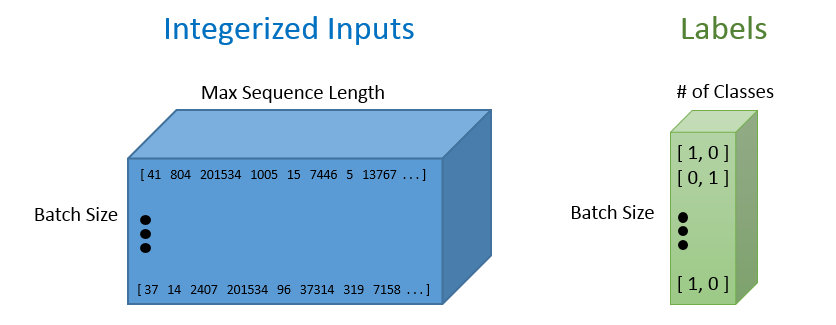
\includegraphics{Images/SentimentAnalysis12.png}
\caption{caption}
\end{figure}

    \begin{Verbatim}[commandchars=\\\{\}]
{\color{incolor}In [{\color{incolor}23}]:} \PY{k+kn}{import} \PY{n+nn}{tensorflow} \PY{k}{as} \PY{n+nn}{tf}
         \PY{n}{tf}\PY{o}{.}\PY{n}{reset\PYZus{}default\PYZus{}graph}\PY{p}{(}\PY{p}{)}
         
         \PY{n}{labels} \PY{o}{=} \PY{n}{tf}\PY{o}{.}\PY{n}{placeholder}\PY{p}{(}\PY{n}{tf}\PY{o}{.}\PY{n}{float32}\PY{p}{,} \PY{p}{[}\PY{n}{batchSize}\PY{p}{,} \PY{n}{numClasses}\PY{p}{]}\PY{p}{)}
         \PY{n}{input\PYZus{}data} \PY{o}{=} \PY{n}{tf}\PY{o}{.}\PY{n}{placeholder}\PY{p}{(}\PY{n}{tf}\PY{o}{.}\PY{n}{int32}\PY{p}{,} \PY{p}{[}\PY{n}{batchSize}\PY{p}{,} \PY{n}{maxSeqLength}\PY{p}{]}\PY{p}{)}
\end{Verbatim}


    Une fois que nous avons notre espace réservé pour les données d'entrée,
nous allons appeler la fonction tf.nn.lookup () afin d'obtenir nos
vecteurs de mots. L'appel à cette fonction renvoie un tensor 3D de
taille de lot de dimensionnalité par longueur de séquence maximale par
dimensions de vecteur de mot. Afin de visualiser ce tenseur 3D, vous
pouvez simplement considérer chaque point de données dans le tensor
d'entrée entier comme le vecteur dimensionnel correspondant auquel il
fait référence.

    \begin{figure}
\centering
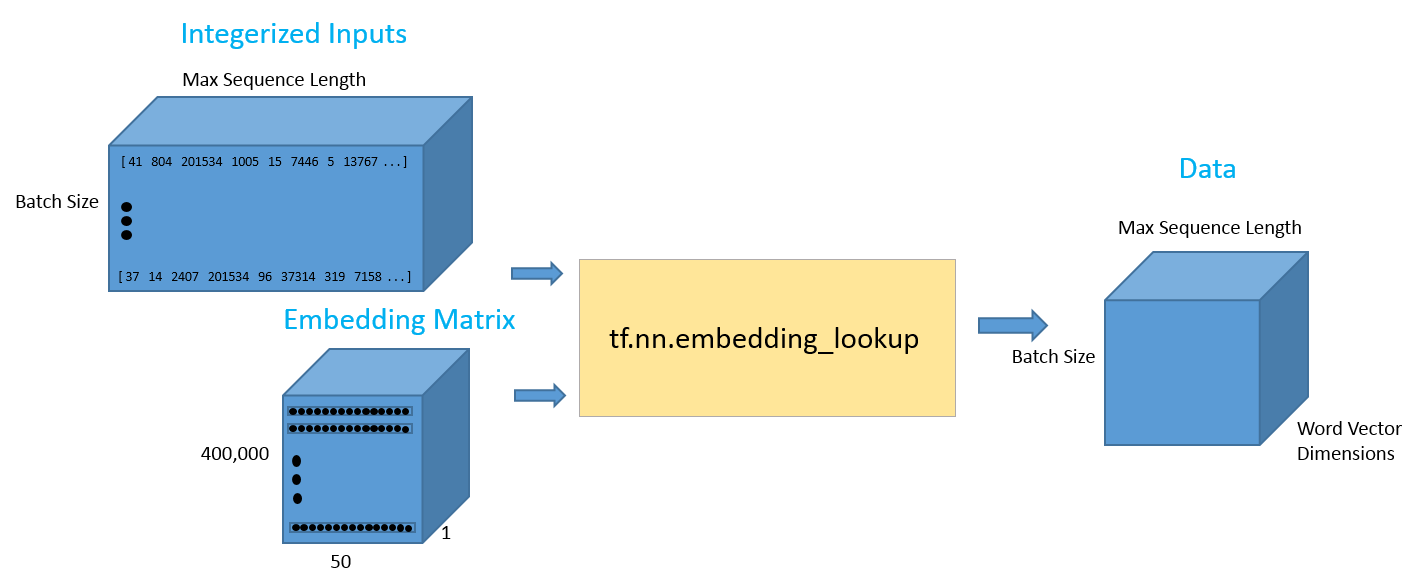
\includegraphics{Images/SentimentAnalysis13.png}
\caption{caption}
\end{figure}

    \begin{Verbatim}[commandchars=\\\{\}]
{\color{incolor}In [{\color{incolor}24}]:} \PY{n}{data} \PY{o}{=} \PY{n}{tf}\PY{o}{.}\PY{n}{Variable}\PY{p}{(}\PY{n}{tf}\PY{o}{.}\PY{n}{zeros}\PY{p}{(}\PY{p}{[}\PY{n}{batchSize}\PY{p}{,} \PY{n}{maxSeqLength}\PY{p}{,} \PY{n}{numDimensions}\PY{p}{]}\PY{p}{)}\PY{p}{,}\PY{n}{dtype}\PY{o}{=}\PY{n}{tf}\PY{o}{.}\PY{n}{float32}\PY{p}{)}
         \PY{n}{data} \PY{o}{=} \PY{n}{tf}\PY{o}{.}\PY{n}{nn}\PY{o}{.}\PY{n}{embedding\PYZus{}lookup}\PY{p}{(}\PY{n}{wordVectors}\PY{p}{,}\PY{n}{input\PYZus{}data}\PY{p}{)}
\end{Verbatim}


    Maintenant que nous avons les données dans le format que nous voulons,
regardons comment nous pouvons nourrir cette entrée dans un réseau LSTM.
Nous allons appeler la fonction tf.nn.rnn\_cell.BasicLSTMCell. Cette
fonction prend un nombre entier pour le nombre d'unités LSTM que nous
voulons. C'est l'un des hyperparamètres qui prendra un certain réglage
pour déterminer la valeur optimale. Nous allons ensuite envelopper cette
cellule LSTM dans un dropout layer pour éviter que le réseau ne fait pas
un sur-apprentissage.

    Enfin, nous allons alimenter la cellule LSTM et le tensor 3D complet des
données d'entrée dans une fonction appelée tf.nn.dynamic\_rnn. Cette
fonction est chargée de dérouler tout le réseau et de créer un chemin
pour que les données circulent à travers le graphe RNN.

    \begin{Verbatim}[commandchars=\\\{\}]
{\color{incolor}In [{\color{incolor}25}]:} \PY{n}{lstmCell} \PY{o}{=} \PY{n}{tf}\PY{o}{.}\PY{n}{contrib}\PY{o}{.}\PY{n}{rnn}\PY{o}{.}\PY{n}{BasicLSTMCell}\PY{p}{(}\PY{n}{lstmUnits}\PY{p}{)}
         \PY{n}{lstmCell} \PY{o}{=} \PY{n}{tf}\PY{o}{.}\PY{n}{contrib}\PY{o}{.}\PY{n}{rnn}\PY{o}{.}\PY{n}{DropoutWrapper}\PY{p}{(}\PY{n}{cell}\PY{o}{=}\PY{n}{lstmCell}\PY{p}{,} \PY{n}{output\PYZus{}keep\PYZus{}prob}\PY{o}{=}\PY{l+m+mf}{0.75}\PY{p}{)}
         \PY{n}{value}\PY{p}{,} \PY{n}{\PYZus{}} \PY{o}{=} \PY{n}{tf}\PY{o}{.}\PY{n}{nn}\PY{o}{.}\PY{n}{dynamic\PYZus{}rnn}\PY{p}{(}\PY{n}{lstmCell}\PY{p}{,} \PY{n}{data}\PY{p}{,} \PY{n}{dtype}\PY{o}{=}\PY{n}{tf}\PY{o}{.}\PY{n}{float32}\PY{p}{)}
\end{Verbatim}


    En remarque, un autre choix d'architecture de réseau plus avancé
consiste à empiler plusieurs cellules LSTM les unes sur les autres.
C'est là que le vecteur d'état caché final du premier LSTM se nourrit
dans le second. Empiler ces cellules est une excellente façon d'aider le
modèle à conserver plus d'informations sur la dépendance à long terme,
mais introduit également plus de paramètres dans le modèle, augmentant
ainsi le temps d'entraînement, le besoin d'exemples d'entraînement
supplémentaires et les risques d'overfitting. Pour plus d'informations
sur la façon dont vous pouvez ajouter des LSTM empilés à votre modèle,
consultez l'excellente
\href{https://www.tensorflow.org/tutorials/recurrent\#stacking_multiple_lstms}{documentation}
du Tensorflow.

    La première sortie de la fonction RNN dynamique peut être considérée
comme le dernier vecteur de hidden state. Ce vecteur sera remodelé puis
multiplié par une matrice de poids final et un terme de biais pour
obtenir les valeurs de sortie finales.

    \begin{Verbatim}[commandchars=\\\{\}]
{\color{incolor}In [{\color{incolor}26}]:} \PY{n}{weight} \PY{o}{=} \PY{n}{tf}\PY{o}{.}\PY{n}{Variable}\PY{p}{(}\PY{n}{tf}\PY{o}{.}\PY{n}{truncated\PYZus{}normal}\PY{p}{(}\PY{p}{[}\PY{n}{lstmUnits}\PY{p}{,} \PY{n}{numClasses}\PY{p}{]}\PY{p}{)}\PY{p}{)}
         \PY{n}{bias} \PY{o}{=} \PY{n}{tf}\PY{o}{.}\PY{n}{Variable}\PY{p}{(}\PY{n}{tf}\PY{o}{.}\PY{n}{constant}\PY{p}{(}\PY{l+m+mf}{0.1}\PY{p}{,} \PY{n}{shape}\PY{o}{=}\PY{p}{[}\PY{n}{numClasses}\PY{p}{]}\PY{p}{)}\PY{p}{)}
         \PY{n}{value} \PY{o}{=} \PY{n}{tf}\PY{o}{.}\PY{n}{transpose}\PY{p}{(}\PY{n}{value}\PY{p}{,} \PY{p}{[}\PY{l+m+mi}{1}\PY{p}{,} \PY{l+m+mi}{0}\PY{p}{,} \PY{l+m+mi}{2}\PY{p}{]}\PY{p}{)}
         \PY{n}{last} \PY{o}{=} \PY{n}{tf}\PY{o}{.}\PY{n}{gather}\PY{p}{(}\PY{n}{value}\PY{p}{,} \PY{n+nb}{int}\PY{p}{(}\PY{n}{value}\PY{o}{.}\PY{n}{get\PYZus{}shape}\PY{p}{(}\PY{p}{)}\PY{p}{[}\PY{l+m+mi}{0}\PY{p}{]}\PY{p}{)} \PY{o}{\PYZhy{}} \PY{l+m+mi}{1}\PY{p}{)}
         \PY{n}{prediction} \PY{o}{=} \PY{p}{(}\PY{n}{tf}\PY{o}{.}\PY{n}{matmul}\PY{p}{(}\PY{n}{last}\PY{p}{,} \PY{n}{weight}\PY{p}{)} \PY{o}{+} \PY{n}{bias}\PY{p}{)}
\end{Verbatim}


    Ensuite, nous définirons des métriques de prédiction et de précision
correctes pour suivre l'évolution du réseau. La formulation de
prédiction correcte fonctionne en examinant l'index de la valeur
maximale des deux valeurs de sortie, puis en vérifiant si elle
correspond aux étiquettes d'apprentissage.

    \begin{Verbatim}[commandchars=\\\{\}]
{\color{incolor}In [{\color{incolor}27}]:} \PY{n}{correctPred} \PY{o}{=} \PY{n}{tf}\PY{o}{.}\PY{n}{equal}\PY{p}{(}\PY{n}{tf}\PY{o}{.}\PY{n}{argmax}\PY{p}{(}\PY{n}{prediction}\PY{p}{,}\PY{l+m+mi}{1}\PY{p}{)}\PY{p}{,} \PY{n}{tf}\PY{o}{.}\PY{n}{argmax}\PY{p}{(}\PY{n}{labels}\PY{p}{,}\PY{l+m+mi}{1}\PY{p}{)}\PY{p}{)}
         \PY{n}{accuracy} \PY{o}{=} \PY{n}{tf}\PY{o}{.}\PY{n}{reduce\PYZus{}mean}\PY{p}{(}\PY{n}{tf}\PY{o}{.}\PY{n}{cast}\PY{p}{(}\PY{n}{correctPred}\PY{p}{,} \PY{n}{tf}\PY{o}{.}\PY{n}{float32}\PY{p}{)}\PY{p}{)}
\end{Verbatim}


    Nous allons définir une standard de cross entropy loss avec une couche
softmax placée au-dessus des valeurs de prédiction finale. Pour
l'optimiseur, nous allons utiliser Adam et le taux d'apprentissage par
défaut de 0,001.

    \begin{Verbatim}[commandchars=\\\{\}]
{\color{incolor}In [{\color{incolor}28}]:} \PY{n}{loss} \PY{o}{=} \PY{n}{tf}\PY{o}{.}\PY{n}{reduce\PYZus{}mean}\PY{p}{(}\PY{n}{tf}\PY{o}{.}\PY{n}{nn}\PY{o}{.}\PY{n}{softmax\PYZus{}cross\PYZus{}entropy\PYZus{}with\PYZus{}logits}\PY{p}{(}\PY{n}{logits}\PY{o}{=}\PY{n}{prediction}\PY{p}{,} \PY{n}{labels}\PY{o}{=}\PY{n}{labels}\PY{p}{)}\PY{p}{)}
         \PY{n}{optimizer} \PY{o}{=} \PY{n}{tf}\PY{o}{.}\PY{n}{train}\PY{o}{.}\PY{n}{AdamOptimizer}\PY{p}{(}\PY{p}{)}\PY{o}{.}\PY{n}{minimize}\PY{p}{(}\PY{n}{loss}\PY{p}{)}
\end{Verbatim}


    Si vous souhaitez utiliser Tensorboard pour visualiser les valeurs de
perte et de précision, vous pouvez également exécuter et modifier le
code suivant.

    \begin{Verbatim}[commandchars=\\\{\}]
{\color{incolor}In [{\color{incolor}29}]:} \PY{k+kn}{import} \PY{n+nn}{datetime}
         
         \PY{n}{tf}\PY{o}{.}\PY{n}{summary}\PY{o}{.}\PY{n}{scalar}\PY{p}{(}\PY{l+s+s1}{\PYZsq{}}\PY{l+s+s1}{Loss}\PY{l+s+s1}{\PYZsq{}}\PY{p}{,} \PY{n}{loss}\PY{p}{)}
         \PY{n}{tf}\PY{o}{.}\PY{n}{summary}\PY{o}{.}\PY{n}{scalar}\PY{p}{(}\PY{l+s+s1}{\PYZsq{}}\PY{l+s+s1}{Accuracy}\PY{l+s+s1}{\PYZsq{}}\PY{p}{,} \PY{n}{accuracy}\PY{p}{)}
         \PY{n}{merged} \PY{o}{=} \PY{n}{tf}\PY{o}{.}\PY{n}{summary}\PY{o}{.}\PY{n}{merge\PYZus{}all}\PY{p}{(}\PY{p}{)}
         \PY{n}{logdir} \PY{o}{=} \PY{l+s+s2}{\PYZdq{}}\PY{l+s+s2}{tensorboard/}\PY{l+s+s2}{\PYZdq{}} \PY{o}{+} \PY{n}{datetime}\PY{o}{.}\PY{n}{datetime}\PY{o}{.}\PY{n}{now}\PY{p}{(}\PY{p}{)}\PY{o}{.}\PY{n}{strftime}\PY{p}{(}\PY{l+s+s2}{\PYZdq{}}\PY{l+s+s2}{\PYZpc{}}\PY{l+s+s2}{Y}\PY{l+s+s2}{\PYZpc{}}\PY{l+s+s2}{m}\PY{l+s+si}{\PYZpc{}d}\PY{l+s+s2}{\PYZhy{}}\PY{l+s+s2}{\PYZpc{}}\PY{l+s+s2}{H}\PY{l+s+s2}{\PYZpc{}}\PY{l+s+s2}{M}\PY{l+s+s2}{\PYZpc{}}\PY{l+s+s2}{S}\PY{l+s+s2}{\PYZdq{}}\PY{p}{)} \PY{o}{+} \PY{l+s+s2}{\PYZdq{}}\PY{l+s+s2}{/}\PY{l+s+s2}{\PYZdq{}}
         \PY{n}{writer} \PY{o}{=} \PY{n}{tf}\PY{o}{.}\PY{n}{summary}\PY{o}{.}\PY{n}{FileWriter}\PY{p}{(}\PY{n}{logdir}\PY{p}{,} \PY{n}{sess}\PY{o}{.}\PY{n}{graph}\PY{p}{)}
\end{Verbatim}


    \section{Hyperparameter Tuning}\label{hyperparameter-tuning}

    Choisir les bonnes valeurs pour vos hyperparamètres est une partie
cruciale de la formation efficace des réseaux de neurone profonds. Vous
constaterez que vos courbes de perte d'entraînement peuvent varier selon
votre choix d'optimiseur (Adam, Adadelta, SGD, etc.), le taux
d'apprentissage et l'architecture réseau. Avec les RNN et les LSTM en
particulier, d'autres facteurs importants incluent le nombre d'unités
LSTM et la taille des vecteurs de mots.

\begin{itemize}
\item
  Learning Rate: RNN sont tristement célèbres pour être diffultes à
  former en raison du grand nombre de pas de temps qu'ils ont. Le taux
  d'apprentissage devient extrêmement important car nous ne voulons pas
  que nos valeurs de poids fluctuent énormément en raison d'un taux
  d'apprentissage élevé, et nous ne voulons pas d'un processus
  d'entraînement lent en raison d'un faible taux d'apprentissage. La
  valeur par défaut de 0,001 est un bon point de départ. Vous devriez
  augmenter cette valeur si la perte d'entraînement change très
  lentement, et diminuer si la perte est instable.
\item
  Optimizer: Il n'y a pas de choix consensuel parmi les chercheurs, mais
  Adam a été très populaire en raison de sa propriété de taux
  d'apprentissage adaptatif (retenez bien optimal learning rates diffère
  avec le choix de l'optimizer).
\item
  Number of LSTM units: Cette valeur dépend en grande partie de la
  longueur moyenne de vos textes d'entrée. Alors qu'un plus grand nombre
  d'unités fournit plus d'expressivité pour le modèle et permet au
  modèle de stocker plus d'informations pour des textes plus longs, le
  réseau prendra plus de temps à s'entraîner et sera coûteux en termes
  de calcul.
\item
  Word Vector Size: Les dimensions pour les vecteurs de mots vont
  généralement de 50 à 300. Une taille plus grande signifie que le
  vecteur est capable d'encapsuler plus d'informations sur le mot, mais
  vous devriez également vous attendre à un modèle plus coûteux en
  calcul.
\end{itemize}

    \section{Training}\label{training}

    L'idée de base de la boucle d'apprentissage est que nous définissons
d'abord une session Tensorflow. Ensuite, nous chargeons un lot de
critiques et leurs étiquettes associées. Ensuite, nous appelons la
fonction \texttt{run} de la session. Cette fonction a deux arguments. Le
premier s'appelle l'argument "fetchs". Il définit la valeur que nous
sommes intéressés par l'informatique. Nous voulons que notre optimiseur
soit calculé car c'est le composant qui minimise notre fonction de
perte. Le deuxième argument est où nous entrons notre
\texttt{feed\_dict}. Cette structure de données est l'endroit où nous
fournissons des intrants à tous nos espaces réservés. Nous devons
nourrir notre batsh de review et notre batsh d'étiquettes (label). Cette
boucle est ensuite répétée pour un nombre déterminé d'itérations
d'apprentissage.

    Au lieu de former le réseau dans ce cahier (ce qui prendra au moins
quelques heures), nous chargerons dans un modèle pré-entraîné.
\href{https://www.tensorflow.org/get_started/summaries_and_tensorboard}{TensorBoard}.

    \begin{Verbatim}[commandchars=\\\{\}]
{\color{incolor}In [{\color{incolor}30}]:}  \PY{n}{sess} \PY{o}{=} \PY{n}{tf}\PY{o}{.}\PY{n}{InteractiveSession}\PY{p}{(}\PY{p}{)}
          \PY{n}{saver} \PY{o}{=} \PY{n}{tf}\PY{o}{.}\PY{n}{train}\PY{o}{.}\PY{n}{Saver}\PY{p}{(}\PY{p}{)}
          \PY{n}{sess}\PY{o}{.}\PY{n}{run}\PY{p}{(}\PY{n}{tf}\PY{o}{.}\PY{n}{global\PYZus{}variables\PYZus{}initializer}\PY{p}{(}\PY{p}{)}\PY{p}{)}
         
          \PY{k}{for} \PY{n}{i} \PY{o+ow}{in} \PY{n+nb}{range}\PY{p}{(}\PY{n}{iterations}\PY{p}{)}\PY{p}{:}
             \PY{c+c1}{\PYZsh{}Next Batch of reviews}
             \PY{n}{nextBatch}\PY{p}{,} \PY{n}{nextBatchLabels} \PY{o}{=} \PY{n}{getTrainBatch}\PY{p}{(}\PY{p}{)}\PY{p}{;}
             \PY{n}{sess}\PY{o}{.}\PY{n}{run}\PY{p}{(}\PY{n}{optimizer}\PY{p}{,} \PY{p}{\PYZob{}}\PY{n}{input\PYZus{}data}\PY{p}{:} \PY{n}{nextBatch}\PY{p}{,} \PY{n}{labels}\PY{p}{:} \PY{n}{nextBatchLabels}\PY{p}{\PYZcb{}}\PY{p}{)}
            
             \PY{c+c1}{\PYZsh{}Write summary to Tensorboard}
             \PY{k}{if} \PY{p}{(}\PY{n}{i} \PY{o}{\PYZpc{}} \PY{l+m+mi}{50} \PY{o}{==} \PY{l+m+mi}{0}\PY{p}{)}\PY{p}{:}
                 \PY{n}{summary} \PY{o}{=} \PY{n}{sess}\PY{o}{.}\PY{n}{run}\PY{p}{(}\PY{n}{merged}\PY{p}{,} \PY{p}{\PYZob{}}\PY{n}{input\PYZus{}data}\PY{p}{:} \PY{n}{nextBatch}\PY{p}{,} \PY{n}{labels}\PY{p}{:} \PY{n}{nextBatchLabels}\PY{p}{\PYZcb{}}\PY{p}{)}
                 \PY{n}{writer}\PY{o}{.}\PY{n}{add\PYZus{}summary}\PY{p}{(}\PY{n}{summary}\PY{p}{,} \PY{n}{i}\PY{p}{)}
         
         \PY{c+c1}{\PYZsh{}    \PYZsh{}Save the network every 10,000 training iterations}
             \PY{k}{if} \PY{p}{(}\PY{n}{i} \PY{o}{\PYZpc{}} \PY{l+m+mi}{10000} \PY{o}{==} \PY{l+m+mi}{0} \PY{o+ow}{and} \PY{n}{i} \PY{o}{!=} \PY{l+m+mi}{0}\PY{p}{)}\PY{p}{:}
                 \PY{n}{save\PYZus{}path} \PY{o}{=} \PY{n}{saver}\PY{o}{.}\PY{n}{save}\PY{p}{(}\PY{n}{sess}\PY{p}{,} \PY{l+s+s2}{\PYZdq{}}\PY{l+s+s2}{models/pretrained\PYZus{}lstm\PYZus{}1.ckpt}\PY{l+s+s2}{\PYZdq{}}\PY{p}{,} \PY{n}{global\PYZus{}step}\PY{o}{=}\PY{n}{i}\PY{p}{)}
                 \PY{n+nb}{print}\PY{p}{(}\PY{l+s+s2}{\PYZdq{}}\PY{l+s+s2}{saved to }\PY{l+s+si}{\PYZpc{}s}\PY{l+s+s2}{\PYZdq{}} \PY{o}{\PYZpc{}} \PY{n}{save\PYZus{}path}\PY{p}{)}
          \PY{n}{writer}\PY{o}{.}\PY{n}{close}\PY{p}{(}\PY{p}{)}
\end{Verbatim}


    \begin{Verbatim}[commandchars=\\\{\}]
saved to models/pretrained\_lstm\_1.ckpt-10000
saved to models/pretrained\_lstm\_1.ckpt-20000
saved to models/pretrained\_lstm\_1.ckpt-30000
saved to models/pretrained\_lstm\_1.ckpt-40000
saved to models/pretrained\_lstm\_1.ckpt-50000
saved to models/pretrained\_lstm\_1.ckpt-60000
saved to models/pretrained\_lstm\_1.ckpt-70000
saved to models/pretrained\_lstm\_1.ckpt-80000
saved to models/pretrained\_lstm\_1.ckpt-90000

    \end{Verbatim}

    \section{Loading a Pretrained Model}\label{loading-a-pretrained-model}

    La precision(accuracy) et Loss sont représentés dans les figures
suivantes

    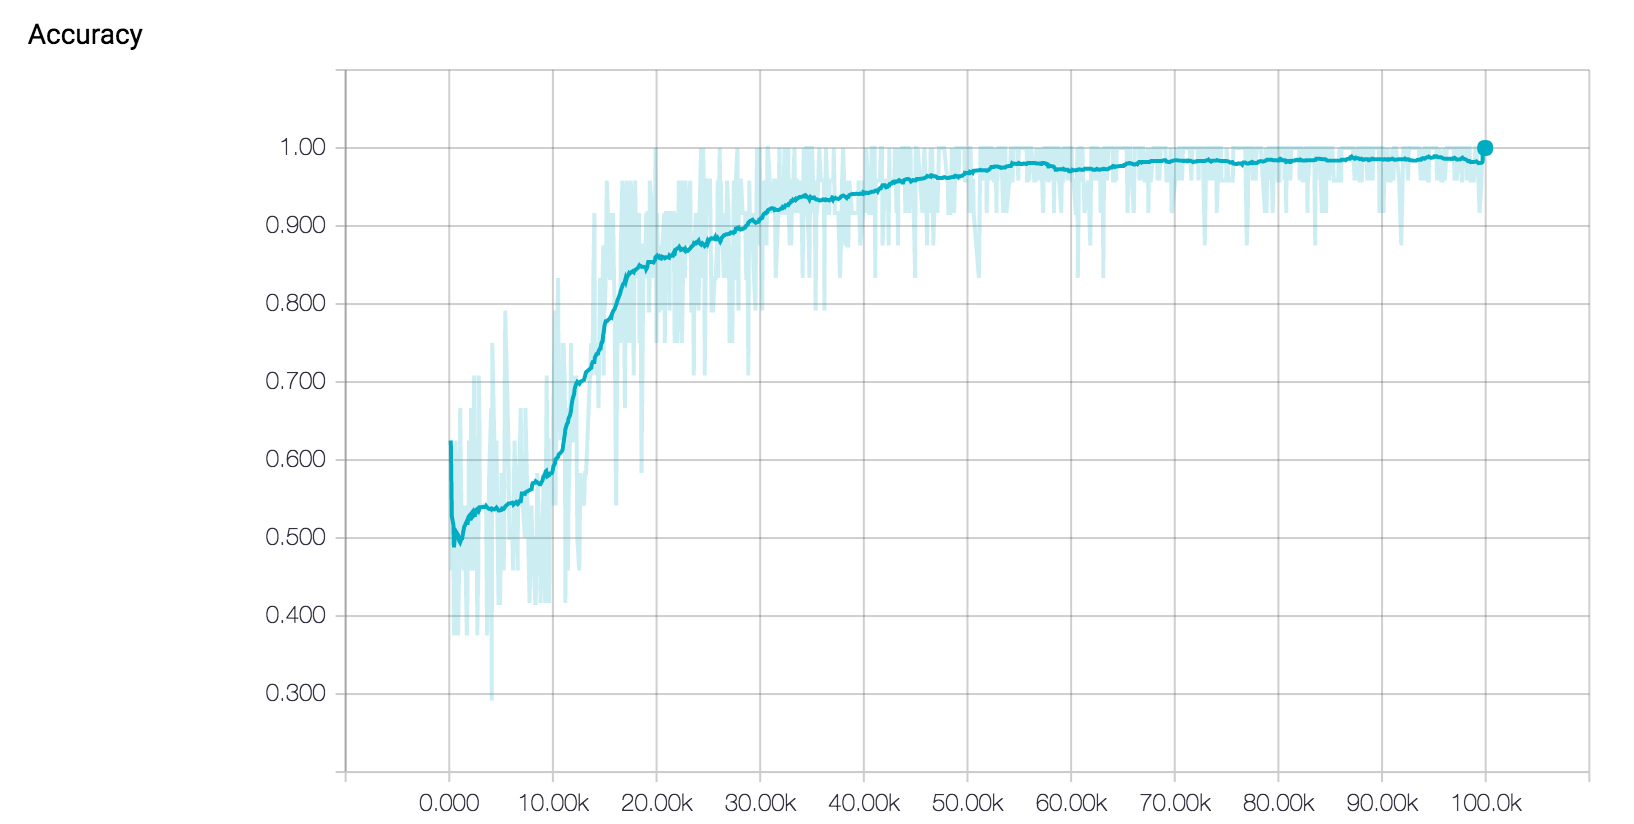
\includegraphics{Images/SentimentAnalysis6.png}
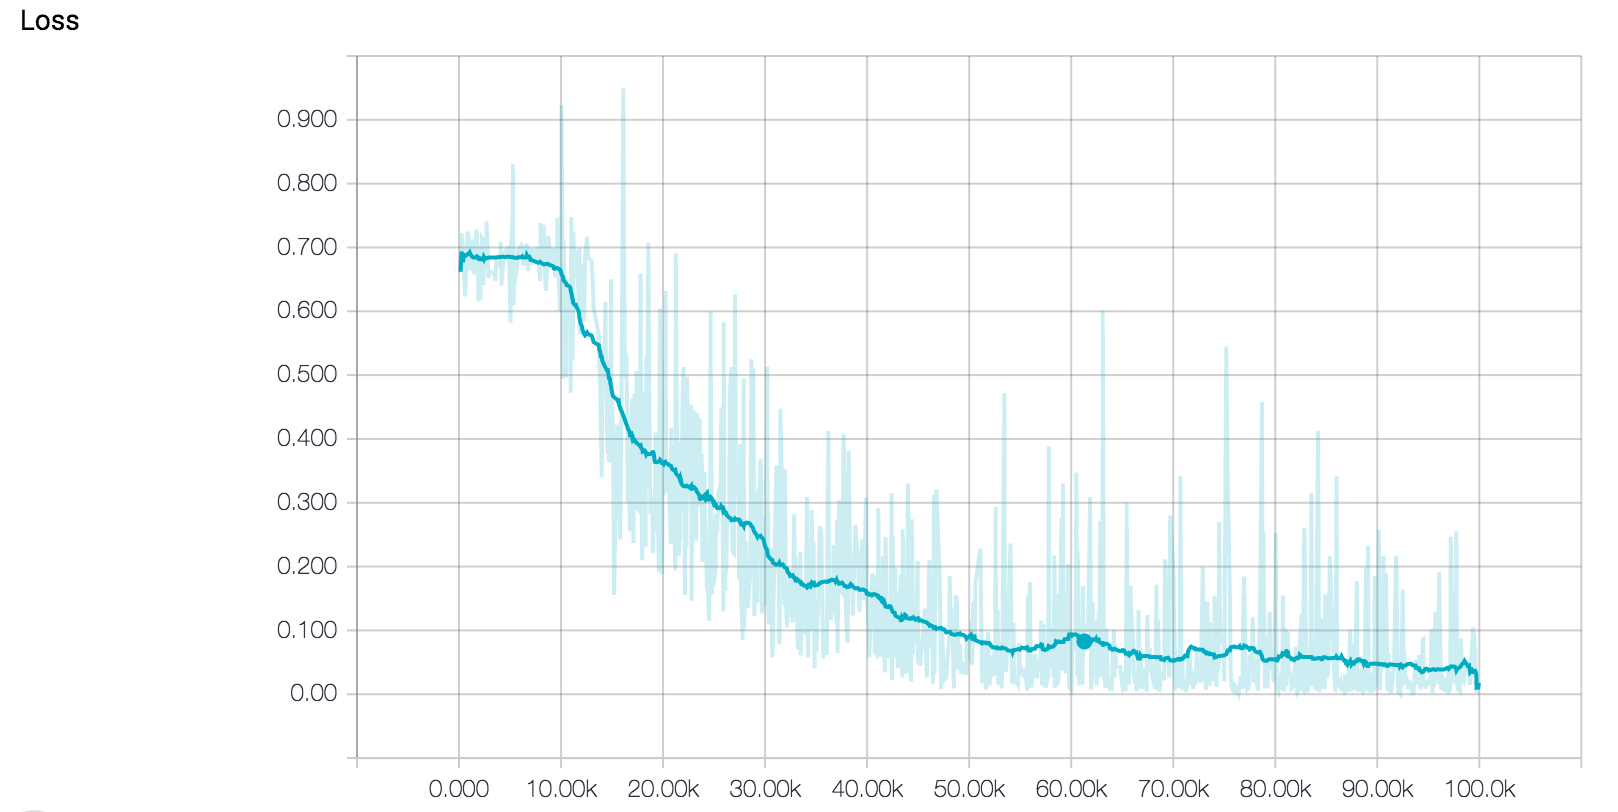
\includegraphics{Images/SentimentAnalysis7.png}

    En regardant les courbes d'entraînement ci-dessus, il semble que la
formation du modèle se passe bien. La perte diminue régulièrement et la
précision approche de 100\%. Toutefois, lors de l'analyse des courbes
d'entraînement, nous devrions également accorder une attention
particulière à la possibilité que notre modèle overfit l'ensemble de
données d'apprentissage. Le surapprentissage est un phénomène courant
dans l'apprentissage automatique où un modèle devient si adapté aux
données d'apprentissage qu'il perd la possibilité de généraliser à
l'ensemble de test. Cela signifie que la formation d'un réseau jusqu'à
ce que vous atteignez 0 perte d'entraînement ne soit pas la meilleure
façon d'obtenir un modèle précis qui fonctionne bien sur des données
qu'il n'a jamais vues auparavant. L'arrêt précoce est une technique
intuitive couramment utilisée avec les réseaux LSTM pour lutter contre
ce problème. L'idée de base est que nous formons le modèle sur notre
ensemble d'entraînement, tout en mesurant de temps en temps ses
performances sur l'ensemble de test. Une fois que l'erreur de test cesse
de diminuer régulièrement et commence à augmenter à la place, vous
saurez arrêter l'entraînement, car c'est un signe que le réseau a
commencé à être overfit.

    Le chargement d'un modèle pré-entraîné implique la définition d'une
autre session Tensorflow, la création d'un objet Saver, puis
l'utilisation de cet objet pour appeler la fonction de restauration.
Cette fonction prend en compte 2 arguments, un pour la session en cours,
et un pour le nom du modèle sauvegardé.

    \begin{Verbatim}[commandchars=\\\{\}]
{\color{incolor}In [{\color{incolor} }]:} \PY{n}{sess} \PY{o}{=} \PY{n}{tf}\PY{o}{.}\PY{n}{InteractiveSession}\PY{p}{(}\PY{p}{)}
        \PY{n}{saver} \PY{o}{=} \PY{n}{tf}\PY{o}{.}\PY{n}{train}\PY{o}{.}\PY{n}{Saver}\PY{p}{(}\PY{p}{)}
        \PY{n}{saver}\PY{o}{.}\PY{n}{restore}\PY{p}{(}\PY{n}{sess}\PY{p}{,} \PY{n}{tf}\PY{o}{.}\PY{n}{train}\PY{o}{.}\PY{n}{latest\PYZus{}checkpoint}\PY{p}{(}\PY{l+s+s1}{\PYZsq{}}\PY{l+s+s1}{models}\PY{l+s+s1}{\PYZsq{}}\PY{p}{)}\PY{p}{)}
\end{Verbatim}


    Ensuite, nous allons charger quelques critiques de films de notre
ensemble de test. Rappelez-vous, ce sont des critiques que le modèle n'a
pas été formé et n'a jamais vu auparavant. La précision pour chaque
batch de test peut être vu lorsque vous exécutez le code suivant.

    \begin{Verbatim}[commandchars=\\\{\}]
{\color{incolor}In [{\color{incolor}34}]:} \PY{n}{iterations} \PY{o}{=} \PY{l+m+mi}{10}
         \PY{k}{for} \PY{n}{i} \PY{o+ow}{in} \PY{n+nb}{range}\PY{p}{(}\PY{n}{iterations}\PY{p}{)}\PY{p}{:}
             \PY{n}{nextBatch}\PY{p}{,} \PY{n}{nextBatchLabels} \PY{o}{=} \PY{n}{getTestBatch}\PY{p}{(}\PY{p}{)}\PY{p}{;}
             \PY{n+nb}{print}\PY{p}{(}\PY{l+s+s2}{\PYZdq{}}\PY{l+s+s2}{Accuracy for this batch:}\PY{l+s+s2}{\PYZdq{}}\PY{p}{,} \PY{p}{(}\PY{n}{sess}\PY{o}{.}\PY{n}{run}\PY{p}{(}\PY{n}{accuracy}\PY{p}{,} \PY{p}{\PYZob{}}\PY{n}{input\PYZus{}data}\PY{p}{:} \PY{n}{nextBatch}\PY{p}{,} \PY{n}{labels}\PY{p}{:} \PY{n}{nextBatchLabels}\PY{p}{\PYZcb{}}\PY{p}{)}\PY{p}{)} \PY{o}{*} \PY{l+m+mi}{100}\PY{p}{)}
\end{Verbatim}


    \begin{Verbatim}[commandchars=\\\{\}]
Accuracy for this batch: 91.6666686535
Accuracy for this batch: 91.6666686535
Accuracy for this batch: 66.6666686535
Accuracy for this batch: 79.1666686535
Accuracy for this batch: 79.1666686535
Accuracy for this batch: 75.0
Accuracy for this batch: 75.0
Accuracy for this batch: 75.0
Accuracy for this batch: 87.5
Accuracy for this batch: 83.3333313465

    \end{Verbatim}


    % Add a bibliography block to the postdoc
    
    
    
    \end{document}
